\documentclass[11pt,a4paper]{article}

\usepackage[T1]{fontenc}
\usepackage[utf8]{inputenc}
\usepackage{lmodern}
\usepackage[margin=2.5cm]{geometry}
\usepackage{microtype}
\usepackage{booktabs}
\usepackage{tabularx}
\usepackage{enumitem}
\usepackage{xcolor}
\usepackage{listings}
\usepackage{tikz}
\usetikzlibrary{positioning,arrows.meta,fit}
\usepackage{csquotes}
\usepackage[backend=biber,style=numeric,sorting=none,maxbibnames=5]{biblatex}
\addbibresource{references.bib}
\usepackage[colorlinks=true,linkcolor=blue!50!black,citecolor=blue!50!black,urlcolor=blue!50!black]{hyperref}

\newcommand{\camshaft}{\textsc{camshaft}}
\newcommand{\code}[1]{\texttt{#1}}
\newcolumntype{L}{>{\raggedright\arraybackslash}X}

\lstset{
  basicstyle=\ttfamily\small,
  columns=fullflexible,
  keepspaces=true,
  frame=single,
  framesep=4pt,
  rulecolor=\color{black!30},
  commentstyle=\color{black!55},
  keywordstyle=\color{blue!50!black},
  showstringspaces=false,
  breaklines=true,
}

\title{\camshaft{}: Research Report\\[0.4ex]
\large Language, data-model and interface choices for an event-driven\\
command interpreter underpinning multiphysics packages}
\author{}
\date{November 2026}

\begin{document}
\maketitle

\begin{abstract}
\noindent
This report records the research done before any \camshaft{} code is written.
\camshaft{} is intended to be infrastructure for large multiphysics packages: an
event-driven command interpreter with a user-facing domain-specific language
(DSL), a schema by which users define and store objects, a dispatch system by
which those objects respond to messages, and an application programming
interface (API) that other packages, possibly written in other languages, can
build on.  The report surveys how existing frameworks solve the same problems,
evaluates candidate implementation and scripting languages, and examines the
options for the data model, dispatch, CPU and GPU portability, and the foreign
interface.

The main conclusions are these.  Rust is a sound choice for the core, with one
significant weakness: its GPU story is fragmented and partly dependent on
unstable compiler features.  That weakness can be contained by a design in
which the infrastructure owns memory, placement and scheduling but does not
own kernel compilation.  Lua, embedded through the \code{mlua} crate, is the
best fit for the user-facing language, provided it is confined to the control
plane.  User objects should be stored column-wise in tables whose buffers are
layout-compatible with Apache Arrow, so that they can be handed to any
language and any device without copying.  Dispatch should be dynamic at the
granularity of whole tables and static inside the kernels that process them.
Package developers define their types in definition scripts and users drive
runs with driver scripts; the two are separated by role and privilege, not by
interpreter modes, and configuration objects share the schema of bulk data
but not its storage.
The foundation of the public API should be a small, versioned C interface,
with idiomatic bindings for Rust, C++, Fortran, Python and Julia layered on
top.  Physics packages are expected to be written mostly in C++ with Kokkos.
The design accommodates them well, and they supply the portable
double-precision GPU kernels that Rust cannot yet produce, but they impose
specific obligations on the infrastructure, which Section~\ref{sec:kokkos}
sets out.  Meshes, including adaptive refinement and unstructured
connectivity, fit the table model once it is extended with declared relations
between tables, index spaces spanning tables, and a protocol for meshes that
change during a run (Section~\ref{sec:mesh}).  The infrastructure itself is
a library with a trivial \code{main}, so that it can be hosted by its own
executable, by a statically linked application, or by Python or Julia; the
core is built with Cargo, and bindings and packages in C++ and Fortran with
CMake against an installed library (Section~\ref{sec:build}).
Section~\ref{sec:roadmap} turns these conclusions into a prototype plan whose
early milestones are experiments designed to confirm or overturn them.
\end{abstract}

\tableofcontents
\newpage

%------------------------------------------------------------------------------
\section{Scope and requirements}
\label{sec:requirements}

The project brief can be reduced to eight requirements.  They are numbered
here so that later sections can refer to them.

\begin{enumerate}[label=\textbf{R\arabic*},leftmargin=3em]
  \item \label{req:interp} \textbf{Event-driven command interpreter.}  The
        program is driven by commands and events, not by a fixed main loop
        compiled into the binary.
  \item \label{req:dsl} \textbf{User-facing DSL.}  Users describe problems and
        control runs in a language designed for that purpose.
  \item \label{req:schema} \textbf{Schema for user objects.}  Users (and
        packages) define new kinds of object; the infrastructure stores them.
  \item \label{req:dispatch} \textbf{Dispatch.}  Objects respond to messages,
        through static dispatch, dynamic dispatch, or both.
  \item \label{req:api} \textbf{Extension API.}  Other packages can build on
        or extend the infrastructure.
  \item \label{req:perf} \textbf{Performance from the start.}  The
        infrastructure must never be the bottleneck of a physics package.
  \item \label{req:port} \textbf{Hardware portability.}  The data model must
        work across as many CPU and GPU platforms as possible.
  \item \label{req:lang} \textbf{Language neutrality.}  Physics packages may
        be written in a language other than the infrastructure's.  The
        working assumption is that most will be written in C++ with Kokkos.
        C++ is to be avoided in the infrastructure itself.
\end{enumerate}

Two of these pull against the rest.  \ref{req:perf} and \ref{req:port} favour
static, ahead-of-time, monomorphic code; \ref{req:interp}, \ref{req:dsl},
\ref{req:schema} and \ref{req:lang} favour run-time flexibility.  Most of the
design questions in this report are questions about where to put the boundary
between the two.

\paragraph{A note on the name.}  A camshaft turns one driving rotation into
the precisely timed actuation of many independent parts.  The infrastructure
plays that role for the packages built on it.  The library is
\code{libcamshaft}, and the C interface uses the short prefix \code{cam\_}.

\paragraph{A note on sources.}  Statements about the current state of fast-moving
projects (Rust GPU tooling, WASI, MPI implementations, Lua releases) were
checked against primary sources in November 2026 and are cited.  They will go
stale, and Section~\ref{sec:risks} lists the ones the design is most sensitive
to.  Architectural descriptions of established frameworks are drawn from their
papers and documentation.

%------------------------------------------------------------------------------
\section{Prior art}
\label{sec:prior}

No existing framework meets all eight requirements, but each requirement has
been met somewhere.  Table~\ref{tab:prior} summarises the systems that were
examined, and the paragraphs below draw out what \camshaft{} should take from
them.

\begin{table}[ht]
\centering
\small
\begin{tabularx}{\textwidth}{@{}l l L L@{}}
\toprule
System & Core & User-facing language & Relevant idea \\
\midrule
LAMMPS~\cite{lammps} & C++ & Line-oriented command script & Command interpreter; \enquote{fixes} that declare which hooks they answer \\
MOOSE~\cite{moose} & C++ & Hierarchical input file & Object factory and registry; objects selected by type name at run time \\
Cactus~\cite{cactus} & C, Fortran & Parameter file plus declarative interface files & Schedule bins; language-neutral \enquote{thorns}; declared variables \\
AMReX~\cite{amrex} & C++ & Parameter file & Device-aware containers; lambdas as kernels \\
Parthenon~\cite{parthenon} & C++ on Kokkos & Parameter file & Variables declared with metadata; packed for bulk kernels \\
Kokkos~\cite{kokkos3} & C++ & None (a library) & One kernel source, many back ends; host and device mirrors \\
Legion and Regent~\cite{legion,regent} & C++; Lua and Terra & Regent, embedded in Lua & Data described as regions with declared privileges; Lua as a staging language \\
Charm++~\cite{charm} & C++ & Interface files & Message-driven objects; the runtime owns scheduling \\
Julia~\cite{julia} & Julia & Julia & Multiple dispatch with specialisation \\
\bottomrule
\end{tabularx}
\caption{Systems examined and the idea each contributes.}
\label{tab:prior}
\end{table}

\paragraph{Command interpreters.}  LAMMPS is the clearest precedent for
\ref{req:interp}.  Its input script is executed one command at a time, each
command either changing state or running the simulation, and almost all of its
functionality is supplied by \enquote{styles} registered with the interpreter.
Its weakness is the language: the script syntax grew by accretion, has weak
control flow and no data structures, and users who need more are pushed to the
Python wrapper.  The lesson is to adopt a real language for the front end from
the first day, and not to grow one.

\paragraph{Hooks and schedules.}  LAMMPS fixes, MOOSE's \code{execute\_on}
flags and Cactus schedule bins are the same mechanism under three names.  The
framework defines named points in the life of a run; an object declares which
of them it responds to; the framework calls each object at each point it
declared.  This is already message dispatch, and it is cheap, because the
framework consults the declarations once and builds a call list per hook.
\camshaft{} should generalise it by letting packages define new messages as well
as new receivers.

\paragraph{Declared data.}  Cactus, Parthenon and Legion all require packages
to \emph{declare} their data to the framework: name, type, shape, and (in
Legion) the privileges with which each task accesses it.  In return the
framework can allocate, checkpoint, communicate, and schedule without
package-specific code.  This is the origin of the \enquote{database schema}
in \ref{req:schema}, and Legion shows how far it can be taken: once access
privileges are declared, parallel scheduling can be derived instead of
hand-written.

\paragraph{Language neutrality.}  Cactus is the strongest precedent for
\ref{req:lang}.  Its core (the \enquote{flesh}) is C, and thorns may be
written in C, C++ or Fortran, because everything a thorn exchanges with the
flesh is described in declarative interface files and passed through a C
calling convention.  Frameworks built on C++ templates (AMReX, Kokkos,
Parthenon) get excellent performance but are effectively closed to other
languages: a template cannot be called from Fortran.  \camshaft{} reverses the
arrangement.  The framework is language-neutral, and a Kokkos package is one
of its clients (Section~\ref{sec:kokkos}).

\paragraph{Lua in high-performance computing.}  Regent is implemented as a
language embedded in Lua, using Terra~\cite{terra} to generate low-level code.
Lua runs at program start to build and specialise the program; the generated
code runs without Lua.  This staging pattern (script first, compiled kernels
afterwards) is the model for how \camshaft{} should use Lua.

%------------------------------------------------------------------------------
\section{Implementation language}
\label{sec:language}

\subsection{Candidates}

Table~\ref{tab:languages} compares the candidates against the properties that
matter for infrastructure of this kind.  C++ is included as the baseline that
most existing frameworks chose.

\begin{table}[ht]
\centering
\small
\begin{tabularx}{\textwidth}{@{}l L L L@{}}
\toprule
Language & Strengths for this project & Weaknesses for this project & Role \\
\midrule
Rust & No garbage collector; static and dynamic dispatch both first-class; memory and data-race safety; strong C interoperability in both directions; one toolchain and package manager & GPU ecosystem fragmented; several numerical features unstable; MPI bindings less mature; only one production compiler & \textbf{Core} \\
C & Universal ABI; a compiler on every machine & No safety; weak abstraction; everything by hand & \textbf{Interface language} \\
Zig & Excellent C interoperability; compile-time evaluation; simple cross-compilation & Still pre-1.0; small scientific ecosystem; no borrow checking & Not chosen; nearest alternative \\
Fortran & Best-in-class array kernels; vendor compilers; OpenMP and OpenACC offload & Poor fit for interpreters, registries and systems code & First-class client \\
Julia & Multiple dispatch; strong GPU packages; productive & Runtime, garbage collector and compilation latency make it awkward to embed as a library & Client \\
Chapel & Productive distributed and GPU programming & Small community; hard to embed in other programs & Not chosen \\
Python & Ubiquitous; huge ecosystem & Slow; heavy to embed; import cost at scale on parallel file systems & Client \\
C++ & Kokkos, SYCL, the entire existing ecosystem & Excluded from the core by the brief; templates do not cross language boundaries & Avoided in the core; \textbf{expected language of packages} \\
\bottomrule
\end{tabularx}
\caption{Candidate languages.}
\label{tab:languages}
\end{table}

\subsection{Assessment of Rust}

\paragraph{What Rust gets right for this project.}  The requirements ask for
both kinds of dispatch, and Rust offers both without ceremony: generics and
traits are monomorphised and inlined, and \code{dyn Trait} gives an explicit
virtual table where one is wanted.  Procedural macros can derive schema
descriptions from ordinary type definitions, which removes the need for the
separate interface compilers that Cactus and Charm++ rely on.  Declaring
\code{\#[repr(C)]} types and \code{extern "C"} functions gives exact control
of layout and calling convention, and tools such as \code{cbindgen} generate
the C header from the Rust source~\cite{cbindgen}.  Finally, Rust's aliasing
rules give the optimiser the \enquote{no two mutable references overlap}
guarantee that Fortran compilers have always exploited and C compilers must be
told about with \code{restrict}.

Interest in Rust for software of this kind is growing in the
high-performance computing community.  Lamellar, a distributed tasking
runtime developed in Rust at Pacific Northwest National Laboratory, was the
subject of an invited talk at ISC~2026~\cite{lamellarisc}; its network back
ends still rest on C libraries, and the project describes itself as under
development~\cite{lamellar}.  CEA is developing Krokkos, an experimental Rust
interface to Kokkos whose stated goal is a Rust API over Kokkos views that
exposes no unsafe code to its users~\cite{krokkos}.  Neither is evidence
about performance.  That has to come from measurement, which is what the
early milestones of Section~\ref{sec:roadmap} are for.

\paragraph{What Rust gets wrong, or has not finished.}  Four gaps matter.

\begin{enumerate}
  \item \emph{GPU programming.}  There is no single accepted way to write a
        GPU kernel in Rust.  Section~\ref{sec:gpu} reviews the options; the
        short version is that every one of them is either tied to one vendor,
        limited in precision, or dependent on an unstable compiler.
  \item \emph{Unstable numerical features.}  Portable SIMD
        (\code{std::simd}) is still available only on the nightly
        compiler~\cite{portablesimd}.  The same is true of automatic
        differentiation (\code{std::autodiff}, built on
        Enzyme~\cite{enzyme}) and GPU offload (\code{std::offload}); both
        became installable through \code{rustup} on nightly during
        2026 but remain experimental~\cite{rustgsoc2026}.
  \item \emph{MPI.}  The established bindings, \code{rsmpi}, document coverage
        of MPI~3.1 and list one-sided communication and parallel I/O as
        unsupported~\cite{rsmpi}.  This is less serious than it looks, as
        Section~\ref{sec:mpi} explains.
  \item \emph{No stable Rust ABI.}  Rust-to-Rust dynamic linking is not
        supported across compiler versions.  The proposed remedy,
        \code{extern "crabi"}, is still an experimental feature
        gate~\cite{crabi}.  Section~\ref{sec:api} treats this as a constraint
        on the plugin design, not as a blocker.
\end{enumerate}

\paragraph{Verdict.}  Rust is viable and is recommended for the core.  None of
the four gaps affects the parts of the system that are hardest to get right
(the interpreter, the schema, the store, the dispatch tables and the foreign
interface), and all four concern the parts that the design can keep at arm's
length.  Zig would be the fallback if Rust proved unworkable, but its pre-1.0
status makes it the riskier choice for infrastructure meant to last.

\paragraph{Policy on unstable features.}  The core should build on stable
Rust.  Nightly-only features may be used behind Cargo feature flags in
optional crates, never in the public interface.

%------------------------------------------------------------------------------
\section{The user-facing language}
\label{sec:dsl}

\subsection{Embedded or external}

There are two ways to provide a DSL.  An \emph{external} DSL has its own
grammar and parser; an \emph{embedded} DSL is a library of functions and
conventions inside an existing general-purpose language.  The history of
scientific input formats argues strongly for embedding.  External formats
start declarative, then acquire variables, then arithmetic, then loops, then
functions, and end as poorly specified programming languages.  Embedding
starts with a complete, documented, debugged language and restricts it.

The recommendation is an embedded DSL, with one safeguard: the interpreter
must not be the only way in.  Every command the DSL can issue should be an
ordinary call in the public API (Section~\ref{sec:api}), so that the DSL is
one client among several and could be replaced, or accompanied by a second
front end, without touching the core.

\subsection{Candidate host languages}

\begin{table}[ht]
\centering
\small
\begin{tabularx}{\textwidth}{@{}l L L@{}}
\toprule
Language & For & Against \\
\midrule
Lua 5.5 & Tiny, portable ANSI C; designed for embedding; 64-bit integers and floats; coroutines; tables double as a configuration format & One-based indexing surprises some users; small standard library \\
LuaJIT & Much faster than the reference interpreter; excellent foreign function interface & Frozen at Lua~5.1 semantics; no tagged releases; narrower platform coverage \\
Luau & Gradual types; sandboxing; actively developed & A dialect; implemented in C++ \\
Python & Familiar to nearly every scientist & Heavy; start-up and import cost; embedding fixes the interpreter version for every package \\
Rhai, Rune & Pure Rust; simple to embed & Small communities; unfamiliar to users; slower than Lua \\
Scheme (Steel) & Pure Rust; macros make DSLs easy & Syntax is a barrier for the intended users \\
Tcl & Long history as a simulation command language & Dated; string-based semantics \\
\bottomrule
\end{tabularx}
\caption{Candidate host languages for the DSL.}
\label{tab:script}
\end{table}

\subsection{Recommendation: Lua through \texttt{mlua}}

Lua is recommended.  It was designed to be embedded in a host program and to
describe data; a Lua table is simultaneously a record, an array and a
configuration block, so a declarative input deck and a script with loops are
the same kind of file.  Coroutines map naturally on to an event-driven
interpreter: a script can yield while the simulation advances and be resumed
when an event fires.  The interpreter is a few hundred kilobytes and has no
start-up cost worth measuring, which matters when it is launched on every MPI
rank.

The \code{mlua} crate provides the Rust binding.  Its current release, 0.12.2
(October 2026), supports Lua~5.1 to 5.5, LuaJIT and Luau behind feature
flags, can compile the chosen Lua from vendored source so that there is no
system dependency, and supports asynchronous Rust functions as Lua
coroutines~\cite{mlua}.  Lua~5.5 has been supported since release 0.11.6
(January 2026).  Because one binding covers all the dialects, the
choice between them can be deferred and even left to the person building the
package.

\paragraph{Which Lua.}  The default should be the reference implementation,
for three reasons: it has true 64-bit integers, which matter for object
identifiers and counts; it compiles anywhere there is a C compiler; and it is
the version the language's documentation describes.  Of its versions,
Lua~5.5~\cite{lua55} is the one to adopt.  It was released in December 2025,
and the Lua team has stated that 5.4.9 (August 2026) is the last release of
Lua~5.4~\cite{luaversions}.  LuaJIT is faster, but it publishes rolling
releases with no tagged versions, its maintained branch accepts only limited
new features~\cite{luajitstatus}, and it remains at the Lua~5.1 language
level.  Its speed is irrelevant if the next principle is followed.

\paragraph{Lua stays out of the hot path.}  The rule that makes a scripting
language compatible with \ref{req:perf} is that the script decides
\emph{what} is computed and never performs the computation.  Lua should
execute a number of operations proportional to the number of commands, tables
and time steps, never to the number of cells or particles.  A user-supplied
expression that must be evaluated per element (an initial condition, a source
term) is the one place this is hard, and there are three acceptable answers:
evaluate it once on the host to fill a column; translate a restricted
expression into a kernel; or require a compiled plugin.  Calling back into Lua
from inside a kernel is not acceptable, and is impossible on a GPU.

\subsection{Definition scripts and driver scripts}
\label{sec:scripts}

Two kinds of people write \camshaft{} scripts.  The developer of a mesh or
physics package writes scripts that \emph{define} things: the package's types
and their fields, its configuration objects and parameters, its messages, and
the compiled kernel that answers each message.  The user of those packages
writes scripts that \emph{drive} a run: they create objects of types that
already exist, set parameters and issue commands.  The two have different
owners and different lifetimes.  A definition must stay in step with compiled
code and changes when the package changes; a driver changes with every run.
Cactus draws the same line: each thorn ships declarative files describing
its variables, parameters and schedule, and the user's parameter file can
only set and select~\cite{cactus}.

\paragraph{Separation by role and privilege, not by mode.}  One way to keep
the two apart would be to give the interpreter modes (a definition mode, a
generation mode, an execution mode) and to switch between them.  That is
fragile.  When the meaning or legality of a statement depends on hidden
state, errors come to depend on the order of statements.  LAMMPS input
scripts have this property: its documentation notes that some commands are
valid only when they follow others~\cite{lammpsdocs}.  The separation should
instead be enforced by what a script is \emph{able to call}.  Lua loads each
script with an environment of its own.  A script loaded in the definition
role is given the functions that define, and none that create objects or
advance a run.  A script loaded in the driver role is given the commands,
and cannot alter a type that belongs to a package.  The role is decided by
how the script is loaded, not by anything written in it: a package names its
definition scripts, and the command line names the driver.  Both roles use
the same language and the same \code{cam} module, with different contents.

\paragraph{Creation is not a phase.}  Objects are created during a run as
well as before it: particles are injected, meshes are refined, restart files
are read.  Creating objects is therefore an ordinary command in the event
stream.  There is no \enquote{generation} stage, and a driver may run, create
and run again.

\paragraph{Rules.}  Five rules follow.

\begin{enumerate}
  \item \textbf{The definition script is the single source of truth, and it
        is shipped with the package.}  It is embedded in the plugin, or a
        hash of it is checked when the plugin is loaded, so that the script
        and the compiled code cannot drift apart.  The rule is one source of
        truth per package.  A Rust package compiled into the core may derive
        its definitions from Rust types (Section~\ref{sec:language})
        instead, in which case those types are the source; the registry
        holds the same information either way.
  \item \textbf{Definition scripts can be evaluated offline.}  They need no
        MPI, no device and no simulation, and their only effect is to fill
        the registry.  This is what makes tools possible: generating a typed
        header for C++ or Fortran from a package's definitions, printing
        documentation for its types and parameters, and validating a driver
        script without running it.
  \item \textbf{Bindings are checked once, when the package is loaded.}  A
        compiled kernel declares the columns it reads and writes, with their
        types (Section~\ref{sec:device-memory}).  When the handler is bound,
        the core checks that declaration against the schema and resolves
        names to column handles.  Nothing is looked up or checked inside a
        kernel.  A mismatch is an error at load time that names the package,
        the type and the field.  With a header generated under rule~2, the
        Kokkos adapter's accessors can be typed at compile time as well, and
        the look-ups by name in the sketch of Section~\ref{sec:kokkos}
        disappear.
  \item \textbf{Ownership rules replace a schema freeze.}  Every type belongs
        to a namespace, owned by whoever defined it.  New types may be
        defined at any time, including by a driver in its own namespace.  A
        driver or another package may \emph{add} fields to an existing type
        (a tracer, a diagnostic); because kernels bind to columns by name,
        an added column disturbs none of them.  Nobody may change or remove
        a field of a type they do not own once objects of it exist, and the
        owner does so only through the schema version and a migration
        (Section~\ref{sec:schema-record}).
  \item \textbf{Modes belong to the invocation, not to the script.}  The
        executable, and the library entry points beneath it
        (Section~\ref{sec:build}), offer at least four: run a driver; check
        it, which evaluates the definitions and the driver and validates
        every command without executing any; describe a package, which
        prints its types, fields, parameters and messages; and generate
        headers.
\end{enumerate}

\subsection{What the DSL might look like}
\label{sec:sketch}

The two sketches below are illustrative only.  Between them they show what
the DSL has to express: type definitions, parameters, message bindings and
commands.  In both, \code{cam} is supplied by the environment the script is
loaded with.  The first is a definition script.  It uses the vocabulary of
Section~\ref{sec:vocab} and the record types of Section~\ref{sec:records}.

\begin{lstlisting}[language={[5.3]Lua}]
-- pusher/schema.lua: definition role, shipped with the package.

-- A record type: configuration, held on the host, identical on every rank.
local Species = cam.record("pusher.Species", {
  name   = cam.string,
  charge = cam.f64,
  mass   = cam.f64,
})

-- A bulk type: objects are rows, fields are columns.  Every table of this
-- type carries one Species record as its attributes.
local Particle = cam.type("pusher.Particle", {
  position = cam.vec3(cam.f64),
  velocity = cam.vec3(cam.f64),
}, { attributes = Species })

-- A parameter, a message, and the compiled kernel that answers it.
cam.param("pusher.cfl", cam.f64, { default = 0.5 })
cam.message("pusher.advance")
Particle:answers("pusher.advance", cam.kernel("boris"))  -- checked at load
\end{lstlisting}

The second is a driver script.

\begin{lstlisting}[language={[5.3]Lua}]
-- run.lua: driver role, written by the user.
local pusher = cam.use("pusher")      -- loads the plugin and its definitions

pusher.Particle:extend{ tracer = cam.u32 }   -- adding a field is allowed

local electrons = pusher.Particle:table("electrons",
  { name = "electron", charge = -1.602e-19, mass = 9.109e-31 })
electrons:create(1000000)

-- A handler written in Lua: called once per event, never once per object.
cam.on("step_end", function(ev)
  if ev.step % 100 == 0 then
    cam.write{ tables = {electrons}, format = "hdf5" }
  end
end)

cam.run{ until_time = 1.0e-6, dt = 1.0e-9 }
\end{lstlisting}

The names in the sketches are placeholders, invented for a small example
drawn from particle simulation.  Table~\ref{tab:placeholders} says what each
stands for.  The functions of the \code{cam} module that the sketches call
(\code{cam.type}, \code{cam.record}, \code{answers}, \code{cam.use},
\code{extend}, \code{table}, \code{create}, \code{cam.on}, \code{cam.write},
\code{cam.run} and the rest) are placeholders in the same sense.  They stand
for capabilities this report proposes, not for an interface that has been
designed.

\begin{table}[ht]
\centering
\small
\begin{tabularx}{\textwidth}{@{}>{\raggedright\arraybackslash}p{34mm} L@{}}
\toprule
Name & What it stands for \\
\midrule
\code{pusher} & The example package, and the namespace that owns its definitions.  A \enquote{particle pusher} is the part of a particle simulation that advances each particle's position and velocity over a time step \\
\code{boris} & The compiled kernel, in the package's library, that answers \code{pusher.advance}.  It is named after the Boris algorithm, the usual pusher for charged particles in electric and magnetic fields~\cite{boris} \\
\code{pusher.Particle} & A bulk type.  Each particle is a row, and \code{position} and \code{velocity} are its fields \\
\code{pusher.Species} & A record type holding what all particles of one kind share: a name, a charge and a mass.  The driver supplies the values for the electron, in SI units \\
\code{pusher.cfl} & An example of a package parameter.  It is named after the Courant--Friedrichs--Lewy number, a dimensionless limit on the size of a time step \\
\code{pusher.advance} & A message asking a table of particles to advance by one time step \\
\code{tracer} & A field added by the user, not by the package: a label, say, for following chosen particles through the output \\
\code{electrons} & A table of particles, with a name chosen by the user \\
\code{step\_end} & An event that the core is assumed to emit at the end of every time step \\
\code{schema.lua}, \code{run.lua} & File names, which are arbitrary \\
\bottomrule
\end{tabularx}
\caption{Placeholder names used in the sketches.}
\label{tab:placeholders}
\end{table}

%------------------------------------------------------------------------------
\section{The schema and the store}
\label{sec:schema}

\subsection{Rows or columns}

A \enquote{user object} could be stored as a structure (all of its fields
together, an array of structures) or as a row in a set of parallel columns (a
structure of arrays).  For this project the choice is forced.  SIMD units and
GPUs both want one contiguous array per field; a kernel that touches two
fields out of twenty should not pull the other eighteen through the cache; and
a column of one primitive type is the only data shape that every language and
every device API can receive without translation.  The store should be
columnar.

This is the design that game engines call an entity--component system and
that databases call a column store.  Two mature implementations are worth
studying before writing one: Flecs, written in C~\cite{flecs}, and Bevy's
ECS, written in Rust~\cite{bevyecs}.  Both group objects that have the same
set of fields into one table (an \enquote{archetype}), which is exactly the
unit at which Section~\ref{sec:dispatch} proposes to dispatch.  Neither is
suitable for direct use, since neither manages device memory or distributed
data, but their table layouts and query models are directly applicable.

\subsection{Types, fields, tables, rows and columns}
\label{sec:vocab}

The word \enquote{class} promises more than the store provides, so the terms
are fixed here.

\begin{description}[style=nextline,leftmargin=2em]
  \item[Type.]
        A named list of fields, such as \code{pusher.Particle} in the
        example of Section~\ref{sec:sketch}.  It is a
        description held in the registry and nothing more: it contains no
        data and no behaviour.  The nearest familiar things are a
        \code{struct} declaration and the definition of a database table.
  \item[Field.]
        One named member of a type.  It has a name, an element type
        (\code{f64}, \code{u32}), a shape (a scalar, a fixed-size vector or
        tensor, or a relation to another table) and the metadata listed in
        Section~\ref{sec:schema-record}.
  \item[Table.]
        The storage for objects of one type.  A type may have several
        tables: electrons and ions are two tables of one particle type.  A
        handler is selected by type and invoked once for each table
        (Section~\ref{sec:dispatch}).
  \item[Row.]
        One object.  An object is not a block of memory.  It is an index
        that is valid in every column of its table.
  \item[Column.]
        All the values of one field, across every row of a table, in one
        contiguous buffer.  Columns are what a kernel receives.
\end{description}

\begin{lstlisting}
type pusher.Particle         table "electrons", three rows
  position : vec3(f64)         position  [ x0 y0 z0 | x1 y1 z1 | x2 y2 z2 ]
  mass     : f64               mass      [ m0       | m1       | m2       ]
                                           row 0      row 1      row 2
\end{lstlisting}

\enquote{The mass of particle~1} is \code{mass[1]}.  A row index is not an
identity, because rows are renumbered, compacted and migrated
(Section~\ref{sec:relations}); an object that needs a permanent identity has
a column holding a global identifier.

Table~\ref{tab:oo} relates these terms to the object-oriented ones that
package developers will bring with them, and states where each
correspondence stops.

\begin{table}[ht]
\centering
\small
\begin{tabularx}{\textwidth}{@{}>{\raggedright\arraybackslash}p{27mm} >{\raggedright\arraybackslash}p{36mm} L@{}}
\toprule
Object-oriented term & \camshaft{} term & Where the correspondence stops \\
\midrule
Class & Type & A type describes data only.  There is no inheritance; types are related through declared relations between tables \\
Member variable & Field & Stored as a column, apart from the object's other fields.  There are no private members: any package may use a field by declaring that it reads or writes it \\
Instance & Row & A row has no address and no lifetime of its own.  It is identified by its table and an index that can change \\
Method & Handler bound to a message for a type & Called once per table with a range of rows, not once per object.  The body is a compiled kernel, and there is no per-object virtual call \\
Static member & Table attribute (Section~\ref{sec:records}) & One value shared by all the rows of a table, not by every object of the type \\
Constructor, destructor & Commands that create and delete rows & Bulk operations on a table.  Initial values are written by a handler or by filling columns \\
\bottomrule
\end{tabularx}
\caption{Object-oriented terms and their \camshaft{} counterparts.}
\label{tab:oo}
\end{table}

\subsection{What a schema must record}
\label{sec:schema-record}

A type definition in \camshaft{} is run-time data, created by the DSL or by a
package through the API.  For each type the registry should record:

\begin{itemize}
  \item its namespace, which determines who owns it
        (Section~\ref{sec:scripts}), and its storage class, bulk or record
        (Section~\ref{sec:records});
  \item a stable identifier, derived from the qualified name, so that
        checkpoints and separately compiled plugins agree on it;
  \item for each field, its name, element type, shape (scalar, fixed-size
        vector or tensor) and physical unit, if any;
  \item for each field, placement and life-cycle metadata: whether it lives
        on the host, on a device, or both; whether it is checkpointed; whether
        it is exchanged between MPI ranks;
  \item a schema version, so that old checkpoints can be migrated.
\end{itemize}

Element types should be restricted to fixed-width primitives and fixed-size
arrays of them.  Variable-length and pointer-bearing fields do not survive the
trip to a GPU or across a process boundary, and admitting them would
compromise \ref{req:port} for every user in order to serve a few.  Objects
that need variable-length data can refer to rows in another table.  Such
references are essential for meshes, and Section~\ref{sec:relations} makes
them a declared kind of column, including a variable-length form built from
two fixed-width buffers.

\subsection{Records: configuration objects}
\label{sec:records}

Not everything a package defines is bulk data.  A solver, a material, a
boundary condition and an output request are objects too, but there are few
of them and they mostly hold parameters.  They could be stored as tables
with one row for each instance, so that everything is a table.  That is
rejected, because configuration objects need what the store forbids and use
nothing the store provides.

\begin{itemize}
  \item \emph{They need variable-length data}: names, file paths, lists,
        nested settings, references to functions.  Admitting those to tables
        would complicate renumbering, migration and device mirroring for
        every bulk table.
  \item \emph{They are replicated, not partitioned.}  Every MPI rank holds
        an identical copy, whereas a table is divided among ranks, with
        owners and ghosts.
  \item \emph{No kernel loops over them.}  Device buffers, alignment and
        spare capacity are pointless for three instances that are read once
        per event.
\end{itemize}

Existing frameworks keep the same division: Cactus between a thorn's
parameters and its grid variables, MOOSE between its objects and its
variables, Parthenon between a package's parameters and its
fields~\cite{cactus,moose,parthenon}.  What \camshaft{} can add is one schema
over both sides.  The design is as follows.

\begin{enumerate}
  \item \textbf{One registry, two storage classes.}  A type is declared
        either as \emph{bulk} or as a \emph{record}.  Objects of a bulk type
        are rows in tables: fixed-width fields only, able to live on a
        device, partitioned among ranks.  Objects of a record type are held
        on the host, replicated on every rank, and may contain strings,
        lists and nested records.
  \item \textbf{Everything else is shared.}  Both kinds use the same
        definition syntax, the same field metadata (name, type, unit,
        default, documentation), stable identifiers, schema versions,
        persistence and introspection.  Both can receive messages: a handler
        bound to a record type is called once for each record.  Records are
        changed only by commands, which every rank processes in the same
        order (Section~\ref{sec:dispatch}), so they stay identical without
        being communicated.  A package's parameters are the fields of a
        record type that has a single instance.
  \item \textbf{What a kernel sees of a record is fixed-width.}  It reaches
        the kernel in one of two ways.  For one record per call (a solver's
        tolerance), the fixed-width fields are passed by value with the
        call, as a small plain structure.  For a look-up per element (cells
        that each hold a material index), the fixed-width fields of a set of
        records are generated into an ordinary bulk table, which rows refer
        to through a relation and which can live on a device.  The generated
        table is rebuilt when its records change, using the version counters
        of Section~\ref{sec:mesh-change}.
  \item \textbf{Tables carry attributes.}  A table may have one record
        attached to it, holding values shared by all of its rows, such as
        the charge and mass of a particle species.  The type declares which
        record type its tables carry, and a handler receives the attributes
        with the batch of rows.
\end{enumerate}

The test for a package developer is whether the number of instances grows
with the size of the problem or with the length of the input file.  The
first is a bulk type and the second is a record.  Materials and species lie
between the two, and for them the answer is a record together with a
generated look-up table.

\subsection{Compatibility with Apache Arrow}

Arrow defines an in-memory layout for columnar data and, more usefully, two
small C structures for handing columns between libraries without copying: the
C data interface~\cite{arrowcdata} and the C device data
interface~\cite{arrowcdevice}.  The second extends the first to buffers that
live in device memory.  It carries a device type and identifier and an
optional synchronisation event, keeps all metadata on the host, and
deliberately uses the same device-type numbering as DLPack~\cite{dlpack}, the
tensor-exchange convention used by the Python array libraries.  Its device
list already includes CUDA, pinned CUDA host memory, ROCm, OpenCL, Vulkan,
Metal, oneAPI and WebGPU.  The specification still describes itself as
experimental.

The recommendation is \emph{not} to build on an Arrow library, since those
bring far more than is needed, but to make \camshaft{} columns layout-compatible
with Arrow's fixed-width and fixed-size-list types and to implement export
through both C structures.  That costs little, because the layout in question
is simply a contiguous aligned buffer, and it means that any tool which speaks
Arrow or DLPack (which includes NumPy, CuPy, PyTorch, cuDF and Julia) can view
\camshaft{} data in place.  It directly serves \ref{req:port} and \ref{req:lang}.

\subsection{Device memory}
\label{sec:device-memory}

Each column should own up to two buffers, one on the host and one on a device,
with flags recording which is current.  This is the pattern Kokkos calls a
dual view~\cite{kokkos3}.  It keeps synchronisation explicit and lazy: a
kernel declares which columns it reads and writes and where it runs, and the
store copies only what is stale.  The cost of getting this wrong is large.
The Rust offload study found that transferring data automatically at every
kernel launch could be more than $400\times$ slower on an AMD MI250X than the
same code with data moved explicitly, once per benchmark~\cite{rustoffload}.

Kernels declaring their reads and writes has a second benefit, taken from
Legion: the scheduler can see which kernels are independent and run them
concurrently without the package author writing any threading code.

\subsection{Persistence}

The schema carries enough information to write and read any table without
package-specific code, and the same holds for records, which are written
with the tables they configure.  HDF5 and ADIOS2 are the obvious targets; both are C
libraries with C interfaces.  Checkpoint and restart should be designed with
the store, not added afterwards, because schema versioning is much easier to
build in than to retrofit.

%------------------------------------------------------------------------------
\section{Events and dispatch}
\label{sec:dispatch}

\subsection{The event model}

Everything that happens in \camshaft{} should be an event: a command arriving
from the DSL, the beginning or end of a time step, a request to write output,
a regridding trigger, a message that one package defines and another answers.
An event has a message identifier, an optional target (a type, a table, a
set of rows or a record) and a small payload.  The interpreter's main loop takes events
from a queue and dispatches them.

In a distributed run, the natural arrangement is for every MPI rank to run
the same interpreter over the same script, so that all ranks process the same
sequence of control events without communicating them.  Event ordering must
therefore be deterministic.  Events that originate on one rank (a local error,
a locally detected condition) need an explicit collective step before they
become global events.

\subsection{The cost of dynamic dispatch, and where to pay it}

An indirect call through a table of function pointers costs a few processor
cycles when the branch predictor guesses the target and tens of cycles when it
does not.  The larger cost is indirect: the compiler cannot inline through
the call, and so cannot vectorise across it.  On a GPU the question does not
arise, since device code generally cannot make indirect calls at all.

Dispatching dynamically \emph{per object} is therefore ruled out by
\ref{req:perf} and \ref{req:port}.  Dispatching dynamically \emph{per table}
is essentially free.  If a table holds a million objects of one type, one
table lookup selects the handler and one indirect call invokes it; the handler
is a compiled kernel that loops over the columns with everything inside the
loop statically resolved, inlined and vectorised.  The dispatch overhead is
amortised over a million elements.

This gives the central rule of the design:

\begin{quote}
\emph{Dispatch is dynamic between kernels and static within them.  A message
is resolved once per table, never once per object.}
\end{quote}

It is the same rule that LAMMPS and MOOSE follow informally, and it is what
makes columnar storage and message dispatch fit together: grouping objects by
type into tables is exactly what turns a million dynamic dispatches into one.

\subsection{Mechanism}

\paragraph{Dynamic layer.}  The registry holds a table mapping
\emph{(message identifier, type identifier)} to a handler.  A handler is a C
function pointer plus a context pointer, which is the one representation that
every language can supply.  Both identifiers are small integers assigned at
registration, so lookup is an array index or a single hash probe.  The lookup
result can be cached in the event's call list, as LAMMPS does, so steady-state
time stepping performs no lookups at all.

Three extensions should be anticipated in the table's design even if they are
not built at first: handlers selected by more than one type (multiple
dispatch, as in Julia~\cite{julia}, for interactions between two kinds of
object); several handlers for one message with a defined order; and handlers
selected by execution device as well as by type.

\paragraph{Static layer.}  Inside the Rust core and inside Rust packages,
handlers are generic functions over traits and are monomorphised.  A Rust
package registers a handler through a generic function that instantiates the
kernel for its concrete column types and stores the resulting function
pointer in the dynamic table.  The package author writes static code; the
registration step is where it becomes dynamically reachable.  Packages in
other languages do the same thing by hand: they compile a kernel and register
its address.

\paragraph{When the type set is closed.}  For messages and types that are all
known when the program is built, the dynamic table can be bypassed entirely
and the compiler allowed to resolve the call.  This is an optimisation to
apply where measurement shows it matters, not a second architecture.

%------------------------------------------------------------------------------
\section{Hardware portability}
\label{sec:gpu}

\subsection{CPUs}

Portability across CPU architectures is not in doubt.  Rust targets x86-64,
AArch64, POWER and RISC-V through LLVM, and Lua's reference implementation is
portable C.  Thread-level parallelism within a kernel is well served by
existing work-stealing libraries.  Explicit SIMD is the weak point: until
\code{std::simd} is stabilised~\cite{portablesimd}, stable Rust offers
auto-vectorisation and architecture-specific intrinsics.  Columnar storage
with aligned buffers is what auto-vectorisation needs, so this is tolerable.

\subsection{GPUs: the options in Rust}

Table~\ref{tab:gpu} lists the ways to run a kernel on a GPU from Rust as of
late 2026.  The classification follows NVIDIA's own survey of the
ecosystem~\cite{cudaoxide}.

\begin{table}[ht]
\centering
\small
\begin{tabularx}{\textwidth}{@{}l L L L@{}}
\toprule
Project & Approach & Hardware & Concern \\
\midrule
wgpu~\cite{wgpu} & WebGPU API; kernels in a shading language & Any GPU with Vulkan, Metal or DirectX~12 & Shading language has no 64-bit floats, except through an extension on Vulkan alone \\
CubeCL~\cite{cubecl} & Rust DSL compiled at run time & CUDA, HIP, everything wgpu reaches, and CPUs & Restricted kernel language; self-described alpha (version 0.11) \\
Rust GPU~\cite{rustgpu} & Compiler back end producing SPIR-V & Vulkan-capable GPUs & Graphics-oriented; nightly compiler \\
cuda-oxide~\cite{cudaoxide} & Compiler back end producing PTX & NVIDIA only & Early-stage research project; one vendor \\
\code{std::offload}~\cite{rustoffload} & In the compiler, on LLVM's offload runtime & NVIDIA and AMD; Intel in progress & Nightly only; experimental \\
Vendor libraries through C & CUDA, HIP, oneAPI, Metal called through bindings & Each vendor's own & One kernel source per vendor \\
\bottomrule
\end{tabularx}
\caption{Routes to GPU execution from Rust, late 2026.}
\label{tab:gpu}
\end{table}

Three observations follow.

\paragraph{Double precision excludes the most portable route.}  WebGPU's
shading language has no 64-bit floating-point type, and Apple's Metal has
none either.  wgpu offers 64-bit floats only as a native extension on its
Vulkan back end, with a warning that they may be many times slower than
32-bit ones~\cite{wgpu}.  Most multiphysics codes need double precision at
least in part.
The wgpu route, which is otherwise the most portable and the most mature, is
therefore unsuitable as the \emph{only} back end, and any design must allow
some kernels to be unavailable on some devices.

\paragraph{The compiler-integrated route is the most promising, and is not
ready.}  \code{std::offload} compiles ordinary Rust functions for the GPU
through the same LLVM machinery that OpenMP offload uses in C++ and Fortran.
A study published in August 2026 reports whole-benchmark run times, on
thirteen kernels ported from the RAJA performance suite, between 32\% faster
and 43\% slower than native HIP on an AMD MI250X and between 11\% faster and
46\% slower than native CUDA on an NVIDIA H100~\cite{rustoffload}.  That is
close enough to be taken seriously.  But the authors describe the work as a
prototype and obtained those results with their own extended compiler, and
support for Intel GPUs is still under development.  The Rust project goal to
finish the module in the second half of 2025~\cite{offloadgoal} was not
completed and was superseded by a broader goal for
2026~\cite{rustgoals2026}, which states that stabilisation will not be
requested during that period~\cite{mlgoal2026}.  There is no commitment
about when, or in what form, it will reach stable Rust.

\paragraph{No Rust option yet matches Kokkos.}  Kokkos gives C++ codes one
kernel source for CUDA, HIP, SYCL and OpenMP, in production, at
scale~\cite{kokkos3}.  Nothing in Table~\ref{tab:gpu} does that today.  This
is the single largest cost of avoiding C++ in the core, and it is the reason
physics packages are expected to keep using Kokkos for their kernels.

\subsection{Recommendation: own the data, not the compiler}

The infrastructure should not commit to any one of these.  It should be
designed so that it does not have to.

\begin{enumerate}
  \item \textbf{The store owns device memory.}  A small device abstraction
        (allocate, free, copy between host and device, synchronise) is
        defined as a table of C function pointers.  It can be implemented
        once per vendor runtime by calling that runtime's C interface, which
        is a few hundred lines per back end and involves no kernel
        compilation, or it can be supplied by a package's own runtime
        (Section~\ref{sec:kokkos-memory}).
  \item \textbf{Kernels are opaque.}  To the infrastructure a kernel is a
        function pointer with a declaration: which columns it reads and
        writes, and on which device type it runs.  The infrastructure
        arranges for the data to be in the right place and calls it.  How the
        kernel was compiled (C++ with Kokkos, Rust with CubeCL, Fortran with
        OpenACC, C with CUDA, Julia) is the package's business.
  \item \textbf{One message may have several kernels.}  The dispatch table is
        keyed by device as well as by type, so a package can supply a CPU
        kernel everywhere and GPU kernels where it has them, and the
        scheduler chooses.
\end{enumerate}

This arrangement satisfies \ref{req:port} in the only way currently open
without C++: by being portable in its data model and neutral about kernel
technology.  It also satisfies \ref{req:lang}, since a kernel written in C++
with Kokkos or in Fortran with OpenACC is registered in the same way as one
written in Rust.  And
it leaves \camshaft{} able to adopt \code{std::offload}, or whatever wins, as an
additional way to produce kernels, without redesign.

For the kernels that \camshaft{} itself needs in order to be tested and
demonstrated, the suggestion is plain Rust on the CPU first, then an
experiment with CubeCL for a cross-vendor GPU path and with
\code{std::offload} on nightly to track its progress.

%------------------------------------------------------------------------------
\section{The public interface}
\label{sec:api}

\subsection{The C ABI as the foundation}

The only binary interface that Rust, Fortran, C, Julia, Python and every
future language can all call and all implement is the platform C ABI.  The
foundation of the \camshaft{} API should therefore be a C interface, with the
following properties.

\begin{itemize}
  \item \textbf{Opaque handles.}  Clients hold handles to tables, types and
        contexts, never pointers to internal structures.
  \item \textbf{Plain data across the boundary.}  Arguments are integers,
        floats, pointers with lengths, and \code{repr(C)} structures whose
        first field is their own size, so that fields can be appended in
        later versions without breaking older clients.
  \item \textbf{Columns as Arrow or DLPack structures.}  Access to stored data
        is given through the interfaces described in
        Section~\ref{sec:schema}.
  \item \textbf{Callbacks as function pointer plus context.}  This is how
        handlers are registered from any language.
  \item \textbf{Errors as return codes.}  A Rust panic must never unwind into
        foreign code; every entry point catches panics and converts them to an
        error code with a retrievable message.
  \item \textbf{Explicit versioning.}  A plugin states the interface version
        it was built against, and the core refuses versions it cannot serve.
\end{itemize}

The interface should be written in Rust as \code{extern "C"} functions, with
the header generated by \code{cbindgen}~\cite{cbindgen}, so that the Rust
source remains the single definition.

\subsection{Layers}

Figure~\ref{fig:arch} shows the proposed layering.  Language bindings are thin
wrappers over the C interface.  The Rust binding is a special case: a Rust
package can be linked statically against the core and use its generic API
directly, with full inlining, or be loaded as a plugin through the C interface
like any other.  The C++ binding is the Kokkos adapter described in
Section~\ref{sec:kokkos}.  The Lua front end is itself a client of the same
API, which keeps it honest: anything the DSL can do, a package can do.

\begin{figure}[ht]
\centering
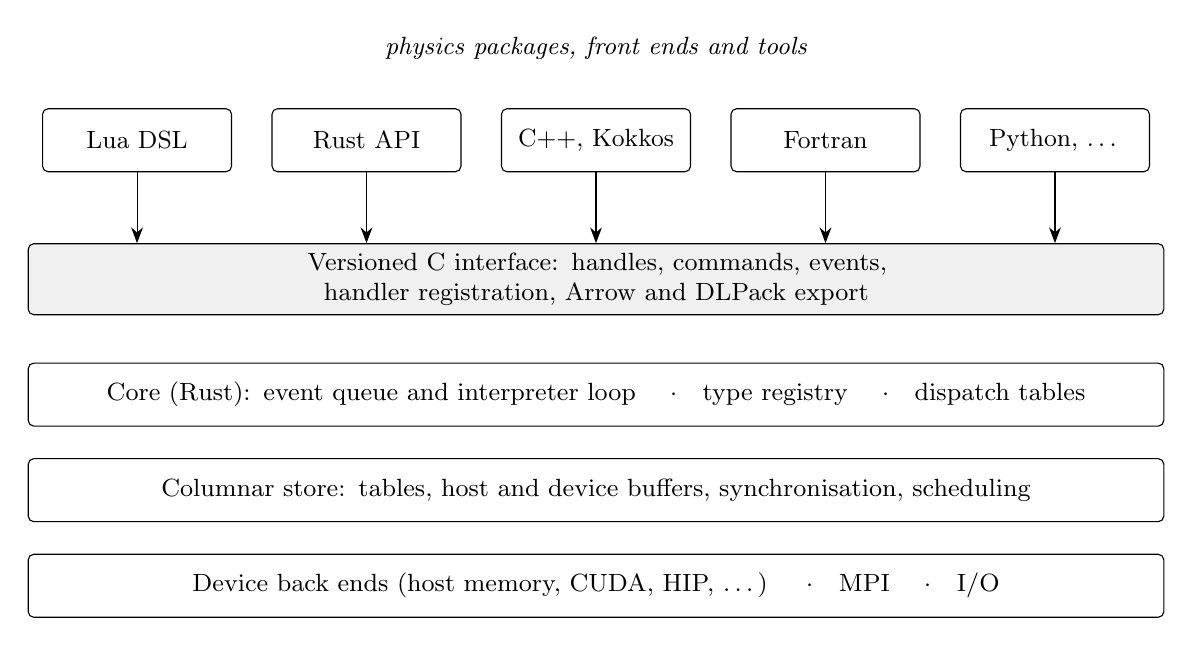
\begin{tikzpicture}[
  box/.style={draw, rounded corners=2pt, minimum height=8mm, align=center, font=\small, inner xsep=6pt},
  wide/.style={box, text width=140mm},
  >={Stealth[length=2mm]},
  node distance=6mm
]
  \node[wide] (core) {Core (Rust): event queue and interpreter loop \quad$\cdot$\quad type registry \quad$\cdot$\quad dispatch tables};
  \node[wide, below=4mm of core] (store) {Columnar store: tables, host and device buffers, synchronisation, scheduling};
  \node[wide, below=4mm of store] (dev) {Device back ends (host memory, CUDA, HIP, \ldots) \quad$\cdot$\quad MPI \quad$\cdot$\quad I/O};
  \node[wide, above=6mm of core, fill=black!6] (cabi) {Versioned C interface: handles, commands, events, handler registration, Arrow and DLPack export};

  \node[box, above=9mm of cabi, minimum width=24mm] (fort) {C++, Kokkos};
  \node[box, left=5mm of fort, minimum width=24mm] (rust) {Rust API};
  \node[box, left=5mm of rust, minimum width=24mm] (lua) {Lua DSL};
  \node[box, right=5mm of fort, minimum width=24mm] (py) {Fortran};
  \node[box, right=5mm of py, minimum width=24mm] (jl) {Python, \ldots};

  \foreach \n in {lua,rust,fort,py,jl} \draw[->] (\n.south) -- (\n.south |- cabi.north);

  \node[above=5mm of fort, font=\small\itshape] {physics packages, front ends and tools};
\end{tikzpicture}
\caption{Proposed layering.  Everything above the shaded bar is a client of
the C interface; a Rust package may alternatively link the core statically.}
\label{fig:arch}
\end{figure}

\subsection{Alternatives considered}

\paragraph{Rust-specific stable ABIs.}  The \code{abi\_stable}~\cite{abistable}
and \code{stabby}~\cite{stabby} crates let Rust libraries exchange richer
types than C allows, with layout checks when a library is loaded.  They solve
Rust-to-Rust plugin loading only, which is not the problem \ref{req:lang}
poses.  They could later be used to make the Rust binding more comfortable.
The language-level proposal, \code{crabi}, remains experimental~\cite{crabi}.

\paragraph{WebAssembly components.}  The WebAssembly component model offers
exactly the language-neutral, versioned, typed interfaces this project wants,
and it is maturing: WASI~0.3, with native asynchronous calls, was released in
June 2026 and is enabled by default in Wasmtime~46~\cite{wasi03}.  It is
nevertheless the wrong tool for the data plane.  A component has its own
linear memory, so passing a column to it means copying; components cannot
reach GPU runtimes or MPI directly; and Fortran toolchain support is thin.  It
is worth revisiting for sandboxed control-plane extensions, where none of
those objections applies.

\paragraph{Remote procedure calls and serialisation.}  Passing messages
between processes would give language neutrality at the price of copying all
data, which \ref{req:perf} rules out for anything but steering and
monitoring.

\subsection{Plugins}

A package should be loadable in two ways: linked into the executable when it
is built, or loaded from a shared library at run time by a DSL command.  In
both cases the package exposes one registration function that receives a
handle to the registry and uses it to define types, messages, handlers and new
DSL commands.  For a package whose definitions are written as a definition
script (Section~\ref{sec:scripts}), the registration function supplies that
script, embedded in the library, and registers the kernels it names; the
core then checks each kernel's declared columns against the schema.  A package may also register initialisation and finalisation
hooks, which the core calls in a defined order relative to MPI and to other
packages; Section~\ref{sec:kokkos-needs} explains why these are needed.
Supporting static linking matters on machines where dynamic loading is
restricted or slow, which includes some of the largest ones.
Section~\ref{sec:build} describes how each configuration is linked and how
the process is started.

%------------------------------------------------------------------------------
\section{C++ and Kokkos physics packages}
\label{sec:kokkos}

The working assumption is that most physics packages built on \camshaft{} will be
written in C++ and will use Kokkos for their kernels.  This section examines
how well the design serves them and what it must provide.  Nothing here has
been tested; milestones M4 and M5 (Section~\ref{sec:roadmap}) exist to test
it.

\subsection{Why the fit is good}

A Kokkos package is a plugin like any other.  It includes the generated C
header, registers handlers with C linkage, and runs Kokkos kernels inside
them.  Three properties of Kokkos make this natural.

\begin{itemize}
  \item \textbf{Kokkos can adopt memory it did not allocate.}  A
        \code{Kokkos::View} constructed from a raw pointer and extents is
        \emph{unmanaged}: it neither copies nor frees the
        memory~\cite{kokkosdocs}.  A handler
        can therefore wrap \camshaft{} columns as views at no cost, on the host or
        on a device.
  \item \textbf{The two data models agree.}  A \camshaft{} column is a contiguous,
        aligned, fixed-width buffer with an optional device copy, which is
        what a view is.  The host and device buffers of
        Section~\ref{sec:schema} were modelled on Kokkos's dual view in the
        first place.
  \item \textbf{The granularity matches.}  Kokkos parallelises a loop over a
        range; \camshaft{} dispatches once per table and passes the handler a
        range of rows.  The handler body is one or a few
        \code{parallel\_for} calls.
\end{itemize}

Kokkos also supplies what Section~\ref{sec:gpu} found missing in Rust: one
double-precision kernel source for CUDA, HIP, SYCL and OpenMP.  For packages
that use it, risk~\ref{risk:gpu} in Section~\ref{sec:risks} largely disappears.
The package keeps access to the libraries built on Kokkos, and it gives up
little: templates cannot cross the C boundary, so nothing from \camshaft{} is
inlined into a kernel, which per-table dispatch never required.

The sketch below shows the shape of a handler.  All \camshaft{} names in it
are invented for illustration, and are explained after it.

\begin{lstlisting}[language=C++]
#include <Kokkos_Core.hpp>
#include <camshaft.h>            // generated C header
#include <camshaft_kokkos.hpp>   // header-only adapter (see below)

extern "C" cam_status advance(cam_batch* batch, void* /*ctx*/) try {
  // Unmanaged views over camshaft columns: no allocation, no copy.
  auto x = cam::view<double*[3]>(batch, "position");
  auto v = cam::view<const double*[3]>(batch, "velocity");
  const double dt = cam_batch_dt(batch);

  Kokkos::parallel_for("advance", x.extent(0), KOKKOS_LAMBDA(const int i) {
    for (int d = 0; d < 3; ++d) x(i, d) += dt * v(i, d);
  });
  return CAM_OK;
} catch (...) {
  return CAM_ERROR_PACKAGE;   // exceptions must not cross the C boundary
}
\end{lstlisting}

\code{advance} is the handler a package would register for a message such as
\code{pusher.advance} in the example of Section~\ref{sec:sketch}.  To keep
the sketch short, its body moves each particle by its velocity and applies
no force; it is not the Boris algorithm.  \code{cam\_batch} stands for what
a handler is given: a range of rows of one table, together with the columns
the handler declared.  \code{cam::view} is the adapter function that wraps
a column as an unmanaged view, and \code{cam\_batch\_dt} reads the time step
from the event's payload.  \code{cam\_status}, \code{CAM\_OK} and
\code{CAM\_ERROR\_PACKAGE} are the return codes of Section~\ref{sec:api}.
\code{camshaft.h} is the generated C header and \code{camshaft\_kokkos.hpp}
is the adapter's header.

\subsection{What the infrastructure must provide}
\label{sec:kokkos-needs}

Each item below is an obligation on \camshaft{} that the earlier sections did not
state, or stated only in general terms.

\paragraph{Runtime life cycle.}  Kokkos can be initialised at most once per
process, and should be initialised after MPI and finalised before MPI is
finalised~\cite{kokkosdocs}.  The
plugin interface therefore needs initialisation and finalisation hooks with a
defined order relative to MPI and to other plugins, in addition to the
registration function of Section~\ref{sec:api}.  \camshaft{} must also tell the
package which device it selected, so that Kokkos is initialised on the same
one.

\paragraph{One Kokkos per process.}  Kokkos keeps global state.  Two plugins
that each link their own copy, or that were built against different versions,
cannot safely share a process.  All Kokkos packages loaded together must use
one shared Kokkos library, and exactly one party must initialise it.  The
simplest rule is that \camshaft{} offers an optional Kokkos adapter which owns
initialisation, and packages depend on that adapter.

\paragraph{Layout.}  A fixed-size-vector column stored in the Arrow manner is
interleaved ($x_0 y_0 z_0\, x_1 y_1 z_1 \ldots$), which Kokkos calls
\code{LayoutRight}.  On GPUs, Kokkos defaults to
\code{LayoutLeft}~\cite{kokkosdocs}.  The
adapter must construct views with the layout stated explicitly.  Whether
interleaved storage is the right default for vector fields, or whether each
component should be its own column, is a performance question for M1 and M5;
the schema should be able to express both.

\paragraph{One source of truth for synchronisation.}  \camshaft{} tracks which of
a column's host and device buffers is current.  Kokkos's own
\code{DualView} does the same.  If a package used both, they would disagree.
Packages must take unmanaged views from \camshaft{} and declare their reads and
writes to it, and must not wrap \camshaft{} memory in a \code{DualView}.

\paragraph{Completion.}  A Kokkos kernel on a GPU may return before the work
is finished.  The scheduler needs to know when a handler's writes are
complete.  The simple contract is that a handler fences before it returns.
The better contract, which allows kernels on independent tables to overlap,
is for the handler to return a completion event; the Arrow device interface
already has a field for one.  The simple contract should come first.

\paragraph{Concurrency.}  Section~\ref{sec:schema} proposed running
independent kernels concurrently.  Kokkos has historically not supported
launching parallel regions from several host threads at once.  Its route to
doing so is separate execution-space instances, and the function that
creates them is still in Kokkos's experimental
namespace~\cite{kokkosdocs}.  Handlers must
therefore be able to declare that they are to be called from one thread at a
time, and that should be the default.  Concurrency between Kokkos kernels can
be revisited later through execution-space instances.

\paragraph{Host threads.}  A Kokkos OpenMP back end and a Rust thread pool
would each try to use every core.  When Kokkos packages are loaded, \camshaft{}
should not run its own data-parallel work at the same time as a handler, and
should let the adapter configure the thread count for both.

\paragraph{Errors.}  A C++ exception that propagates into Rust is undefined
behaviour.  Handlers must catch everything and return an error code, as in
the sketch, and the adapter should provide a wrapper that does this so that
package authors cannot forget.

\paragraph{Build.}  Kokkos packages are built with CMake.  \camshaft{} should
install its C header and library together with a CMake package configuration
file, so that a package finds it with \code{find\_package} and never needs to
invoke Cargo.

\subsection{Who allocates device memory}
\label{sec:kokkos-memory}

For a view to adopt a device buffer, the buffer must have been allocated in a
way the Kokkos back end accepts.  There are two ways to arrange that.

\begin{description}[style=nextline,leftmargin=2em]
  \item[The store allocates through the vendor runtime; Kokkos adopts.]
        This keeps C++ out of the allocation path.  It is straightforward for
        CUDA and HIP, where a pointer from the vendor allocator is valid
        throughout the process.  It is harder for SYCL, where memory belongs
        to a context and Kokkos must be using the same one; that requires
        passing a queue between the two, which has to be verified in M5.
  \item[Kokkos allocates; the store records.]
        The Kokkos adapter implements the device abstraction of
        Section~\ref{sec:gpu} using Kokkos's own allocation and copy
        functions (\code{kokkos\_malloc} and \code{deep\_copy}).  Every back end Kokkos supports then works
        without \camshaft{} knowing anything about it, including ones \camshaft{} has
        no vendor back end for.
\end{description}

Because the device abstraction is a table of C function pointers, both can be
supported, and the recommendation is to do so: vendor back ends for runs
without Kokkos, and the Kokkos-backed allocator as the default whenever the
adapter is loaded.  The second option is the lower-risk route to
\ref{req:port} given the working assumption of this section.

\subsection{The adapter, and the place of C++}

Package authors should not write the view-wrapping, exception-catching and
life-cycle code themselves.  \camshaft{} should ship a small Kokkos adapter: a
header that turns column handles into typed unmanaged views and wraps
handlers, and a small library that owns Kokkos initialisation and implements
the Kokkos-backed allocator.  This is C++ code in the \camshaft{} repository, and
so it qualifies the brief's wish to avoid C++.  This has been accepted, on
the following terms: the adapter is a language binding, of the same standing
as the Fortran or Python bindings; it is optional; and the core neither
contains nor depends on any C++.  The alternative, leaving every package to write its
own adapter, would produce several incompatible ones and would break the
one-Kokkos-per-process rule.

\subsection{Kokkos from Rust}

If packages are in C++ and the core is in Rust, the remaining question is
what Rust packages should use.  Krokkos~\cite{krokkos}, the experimental Rust
interface to Kokkos, is directly relevant: if it matures, Rust and C++
packages could share one runtime, one allocator and one set of back ends
under \camshaft{}.  It should be evaluated alongside CubeCL and
\code{std::offload} in M5.

%------------------------------------------------------------------------------
\section{Process and build model}
\label{sec:build}

The infrastructure drives the execution of the packages built on it, and
those packages are written in several languages.  That raises four practical
questions which the earlier sections left open: what the program's
\code{main} function is, who links the program, how a process containing
several language runtimes is started and stopped, and what build system the
project should use.

\subsection{The infrastructure is a library}

The answer to the first question is that \code{main} should contain almost
nothing.  Everything lives in a library, \code{libcamshaft}, behind the C
interface of Section~\ref{sec:api}.  The library offers one convenience entry
point that takes the command line and runs a script to completion, and
beneath it the individual steps (initialise, load a package, run a script or
a single command, finalise) so that a host can interleave its own work.
Three kinds of host then become possible.

\begin{table}[ht]
\centering
\small
\begin{tabularx}{\textwidth}{@{}l L L@{}}
\toprule
Host & What \code{main} is & When it is used \\
\midrule
Default executable & A Rust \code{main} of a few lines that calls the library & Normal use.  Packages are loaded from shared libraries at run time \\
Custom executable & A C, C++ or Fortran \code{main} that calls the library & Fully static builds; applications that embed \camshaft{} in a larger program \\
Foreign host & None of ours.  Python or Julia loads \code{libcamshaft} and drives it & Interactive work, notebooks, test harnesses, coupling to other tools \\
\bottomrule
\end{tabularx}
\caption{Hosts of the library.}
\label{tab:hosts}
\end{table}

This is the arrangement LAMMPS uses, a library with a trivial \code{main}
and a documented library interface~\cite{lammps}, and it is what makes
\ref{req:lang} hold for the host as well as for packages.  The question
\enquote{Rust's \code{main} or C's?} therefore has no single answer and does
not need one.  A Rust \code{main} is the right default: it is the simplest
thing to build, and a Rust library needs no runtime initialisation when it is
called from a \code{main} written in another language, so nothing is lost in
the other two cases.

\subsection{Starting and stopping the process}

What matters is not who owns \code{main} but the order in which the library
brings the process up and takes it down, since the runtimes in the process
depend on one another.  The library should enforce this sequence:

\begin{enumerate}
  \item initialise MPI, with the thread-support level the loaded packages
        require, unless the host has already done so;
  \item select devices and run the initialisation hooks of language bindings
        (the Kokkos adapter initialises Kokkos here, on the selected device);
  \item load packages and run their registration functions and
        initialisation hooks, in dependency order;
  \item run the interpreter loop;
  \item run finalisation hooks in reverse order, then finalise the bindings,
        then MPI, unless the host owns it.
\end{enumerate}

Each language runtime has its own requirements, and the binding for that
language, not the package author, should meet them.

\begin{description}[style=nextline,leftmargin=2em]
  \item[Fortran.]
        Some compilers need their runtime library initialised explicitly when
        the main program is not Fortran.  Intel's documentation, for example,
        prescribes calls to \code{for\_rtl\_init\_} and
        \code{for\_rtl\_finish\_} and a link option to suppress the Fortran
        main~\cite{intelmixed}.  The Fortran binding's hooks are the place for
        this.
  \item[C++ and Kokkos.]
        Section~\ref{sec:kokkos-needs} covered Kokkos.  Static constructors
        and destructors in C++ packages run when the shared library is loaded
        and unloaded; packages should not depend on their order.
  \item[Julia.]
        Either Julia is the host and calls the library, or a Julia binding
        starts the Julia runtime in its initialisation hook and Julia
        functions are registered as handlers through C-callable function
        pointers.  Compiling Julia packages ahead of time into shared
        libraries is possible with JuliaC, on Julia~1.12 or later, but the
        trimming that keeps such libraries small is still an experimental
        compiler feature~\cite{juliac}.
  \item[Python.]
        The same two options: Python as host, or an embedded interpreter
        started by a binding.  The first is much the more common need.
\end{description}

Three process-wide rules follow from sharing a process.  No package may
terminate the process itself; a fatal error is returned to the library, which
aborts through MPI so that every rank stops.  Signal handlers are installed
only by the library, since several of the runtimes above would otherwise
compete for them.  And interactive input is read on one rank only and
broadcast, so that the deterministic event ordering of
Section~\ref{sec:dispatch} is preserved.

\subsection{Linking}

\paragraph{The default configuration needs no mixed-language link.}  When
packages are plugins, each is a shared library linked by the tool that suits
its language, and that tool adds the language's own runtime libraries
(Table~\ref{tab:link}).  The only things shared between them are the C header
and \code{libcamshaft} itself.  Because Rust's standard library is linked
\emph{inside} \code{libcamshaft}, the library presents itself to every other
language as an ordinary C library with no visible Rust dependency.

\begin{table}[ht]
\centering
\small
\begin{tabularx}{\textwidth}{@{}L L@{}}
\toprule
Artefact & Linked by \\
\midrule
\code{libcamshaft} (shared and static) and the default executable & The Rust compiler, which invokes the C compiler driver, which invokes the system linker \\
Kokkos adapter; C++ packages & CMake, through the C++ compiler or the MPI wrapper for it \\
Fortran packages & The Fortran compiler driver or its MPI wrapper \\
Julia and Python packages & Nothing.  They load \code{libcamshaft} and register function pointers at run time \\
\bottomrule
\end{tabularx}
\caption{Who links what in the default, dynamic configuration.}
\label{tab:link}
\end{table}

The choice of linker proper is not a design decision.  The Rust compiler
delegates to the C compiler driver, and since version 1.90 uses LLD by
default on x86-64 Linux~\cite{rust190lld}; both can be overridden in Cargo's
configuration.  On systems where MPI and vendor libraries are supplied
through compiler wrappers, Cargo should be pointed at the wrapper as its
linker driver.

\paragraph{One copy of the core.}  A process must contain exactly one copy
of the core's state.  The executable and every plugin must therefore resolve
the C interface to the same \code{libcamshaft}, which is why it should normally
be a shared library that all of them link against, with a versioned name.

\paragraph{Rust packages.}  A Rust package has two routes, and they differ
in what is built.  As a plugin it is a shared library that talks to the core
through the C interface like any other; it carries its own copy of Rust's
standard library, which is harmless because only C types cross the boundary.
To use the generic Rust interface with full inlining
(Section~\ref{sec:dispatch}), it must instead be compiled by Cargo
\emph{together with} the core into one artefact, because Rust has no stable
ABI between separately compiled libraries.  In practice that means a small
\enquote{distribution} crate that depends on the core and on the chosen Rust
packages and produces the \code{libcamshaft} that everything else links against.

\paragraph{The static configuration.}  Some large machines discourage or
forbid dynamic loading.  There the whole program is one executable, and the
mixed-language link is unavoidable.  CMake should perform it, since it
computes the runtime libraries each language implicitly needs and links with
the appropriate driver.  Its inputs are the static \code{libcamshaft}, the
packages as static libraries, and a \code{main}.  Three points need care.

\begin{itemize}
  \item \emph{Only one Rust static library per link.}  A Rust static library
        contains the standard library and does not hide its internal symbols,
        so two of them in one link can conflict or silently override each
        other; the compiler options that would hide those symbols are still
        unstable~\cite{ruststaticlib}.  All Rust code in a
        static build must go through the single distribution crate described
        above.
  \item \emph{Registration must be explicit.}  Without dynamic loading there
        is nothing to find a package's registration function.  Relying on
        static constructors fails, because a linker omits archive members
        that nothing refers to.  The build should generate a table of
        registration functions from the list of configured packages and pass
        it to the library, as Cactus generates its thorn
        list~\cite{cactus}.
  \item \emph{The Rust static library has system dependencies} that the
        final link must name.  The Rust compiler can print them, and the
        installed CMake configuration file should record them.
\end{itemize}

\paragraph{One of each runtime.}  In either configuration a process should
contain one MPI library, one Kokkos, one OpenMP runtime and one C++ standard
library.  Two OpenMP runtimes in one process, typically one from a Fortran
compiler and one from a C++ compiler, is a well-known source of crashes and
oversubscription.  The build cannot fully prevent this, but the library can
detect the common cases when a package is loaded and refuse it with a clear
message.

\paragraph{Optimisation across languages.}  Link-time optimisation across
the Rust and C++ boundary is possible when both compilers share an LLVM
version, but the design does not need it: the boundary is crossed once per
table, not once per element.

\subsection{Build system}

\begin{table}[ht]
\centering
\small
\begin{tabularx}{\textwidth}{@{}l L L@{}}
\toprule
Option & For & Against \\
\midrule
Cargo only & Native to Rust; dependency management; testing & No install step for libraries and headers; no Fortran; knows nothing of Kokkos, MPI wrappers or GPU toolchains; build scripts can call other tools but that makes Cargo the outer build for C++ developers \\
CMake only & Native to Kokkos and to most scientific C++ and Fortran; computes mixed-language links & Rust development through CMake loses much of what Cargo provides \\
Meson & First-class support for Rust alongside C, C++ and Fortran & Kokkos and its ecosystem publish CMake packages; less familiar in this field \\
Bazel or Buck & Hermetic multi-language builds & Heavy; alien to supercomputer environments \\
Cargo and CMake, split by ownership & Each community keeps its own tool; neither build invokes the other in normal use & Two systems to maintain; the installed interface between them must be kept exact \\
\bottomrule
\end{tabularx}
\caption{Build-system options.}
\label{tab:buildsys}
\end{table}

Cargo is sufficient for the core and insufficient for the project.  The
recommendation is the last row of Table~\ref{tab:buildsys}.

\begin{description}[style=nextline,leftmargin=2em]
  \item[The core is a pure Cargo workspace.]
        It contains the core, the C interface, the Lua front end (Lua itself
        is compiled from vendored source by \code{mlua}, needing only a C
        compiler), the Rust interface and the default executable.
        \code{cargo build} and \code{cargo test} work with no other tool.
  \item[Installation is an explicit, separate step.]
        Cargo does not install libraries.  \code{cargo-c} builds the shared
        and static libraries, generates the header and a pkg-config file, and
        installs them with correct library versioning~\cite{cargoc}.  The
        installation must also include a CMake package configuration file and
        the \emph{source} of the Fortran interface module, since compiled
        Fortran module files are specific to one compiler.
  \item[Bindings and packages in C++ and Fortran use CMake.]
        They find an installed \camshaft{} with \code{find\_package} and link to
        it as an imported target.  They never invoke Cargo and need no Rust
        toolchain.
  \item[Inside the repository, CMake can build the core too.]
        The adapter's CMake project can use Corrosion, which imports a Cargo
        crate as a CMake target~\cite{corrosion}, so that a C++ developer
        working on the adapter builds everything with one command.  This is
        a convenience; the installed interface remains the contract.
  \item[Julia and Python need no build integration.]
        They load the installed library.  Each binding is an ordinary package
        in its own ecosystem.
  \item[Distribution is through Spack.]
        Spack is how supercomputing sites install software and already
        understands both Cargo and CMake packages~\cite{spack}.
\end{description}

One number must be shared by all of this: the interface version.  It should
be defined once, in the Cargo manifest, and propagated from there to the
header, the library's versioned name, the pkg-config and CMake files, and the
check that the core performs when a plugin registers.

The repository layout that follows from these choices is sketched below.

\begin{lstlisting}
camshaft/
  Cargo.toml            workspace
  crates/
    camshaft-core/      registry, store, events, dispatch
    camshaft-capi/      the C interface; header generated from here
    camshaft-lua/       Lua front end
    camshaft/           Rust interface and default executable
    camshaft-dist/      distribution crate: core + compiled-in Rust packages
  bindings/
    kokkos/             CMake; header-only adapter and small library
    fortran/            CMake; interface module source
    python/  julia/     packages in their own ecosystems
  examples/             one small package per language
  research/             this report
\end{lstlisting}

\subsection{Consequences for the design}

\begin{enumerate}
  \item The C interface gains host entry points: a run-to-completion call
        and the individual initialise, load, run and finalise steps, each
        usable when the host already owns MPI.
  \item Every binding has initialisation and finalisation hooks of its own,
        distinct from those of packages, and the library fixes their order.
  \item The library accepts a table of statically linked registration
        functions as an alternative to loading shared libraries.
  \item The interface version is checked at registration, and the library
        checks for duplicated runtimes when loading a package.
  \item Installation produces the shared and static libraries, the header,
        pkg-config and CMake files, and the Fortran module source.
\end{enumerate}

%------------------------------------------------------------------------------
\section{Distributed memory}
\label{sec:mpi}

MPI remains the only distributed-memory layer available on every
high-performance machine, and \camshaft{} must use it.  The state of the Rust
bindings (Section~\ref{sec:language}) matters less than it seems, for two
reasons.

First, MPI~5.0, approved in June 2025, standardises the ABI: one header and
one set of type and constant definitions, valid for every conforming
implementation~\cite{mpi50,mpiabi}.  MPICH has implemented it since version
5.0.0, released in February 2026~\cite{mpich5}.  Open MPI has added it for
its 6.0 series, which had not been released when this was written, and so
far for C only: its change log notes that the Fortran bindings are not yet
covered~\cite{ompi6}.  That gap does not affect a binding from Rust, which
uses the C interface.  Against a standard
ABI, a Rust binding no longer needs to discover each implementation's
definitions when it is built; the interface can be declared once.  The part of
MPI that an infrastructure layer needs (communicators, non-blocking
point-to-point, collectives, and parallel I/O via a library) is small enough
to bind directly.

Second, the design already hides MPI.  Packages do not call MPI; they declare
which columns are exchanged, and the store performs the exchange.  MPI
therefore sits behind one internal interface and could be supplemented later
by another transport without affecting packages.

The recommendation is to begin with \code{rsmpi}~\cite{rsmpi} for speed of
prototyping, behind an internal trait, and to plan a thin direct binding to
the MPI~5.0 ABI once implementations of it are widespread.

%------------------------------------------------------------------------------
\section{Meshes}
\label{sec:mesh}

Meshes are the most demanding data the infrastructure will hold, and a
package devoted to mesh generation is expected to be built on it.  This
section examines whether the table model of Section~\ref{sec:schema} is
adequate for structured, adaptive and unstructured meshes, and what has to be
added.  The conclusion is that the model is adequate with three additions:
\emph{relations} between tables as a declared kind of column, \emph{index
spaces} that span several tables, and a protocol for \emph{change}, since
adaptive meshes alter the number and identity of rows during a run.

\subsection{Prior art}

\begin{table}[ht]
\centering
\small
\begin{tabularx}{\textwidth}{@{}l L L@{}}
\toprule
System & Mesh kind & Representation \\
\midrule
AMReX~\cite{amrex} & Patch-based structured AMR~\cite{bergercolella} & Levels of rectangular boxes of varying size; connectivity implicit within a box \\
Parthenon~\cite{parthenon} & Block-based structured AMR & Tree of blocks of identical size, packed into one array for bulk kernels \\
p4est~\cite{p4est} & Forest of octrees & Leaves stored as a sorted array along a space-filling curve; no pointers \\
PETSc DMPlex~\cite{dmplex} & Unstructured, any dimension and cell type & All entities numbered in one index space; adjacency stored as offset and index arrays \\
MOAB~\cite{moab} & Unstructured & Entities grouped by type in contiguous ranges; data as \enquote{tags}; arbitrary entity sets \\
PUMI~\cite{pumi} & Unstructured, adaptive & Full adjacencies; every entity classified on a geometric model entity \\
Omega\_h~\cite{omegah} & Simplex, adaptive, on GPUs & Arrays only, on Kokkos; adaptation as bulk array operations \\
Conduit Blueprint~\cite{blueprint} & All of the above & A naming convention for describing mesh arrays in memory, not a data structure \\
\bottomrule
\end{tabularx}
\caption{Mesh systems examined.}
\label{tab:mesh}
\end{table}

Three lessons follow from Table~\ref{tab:mesh}.

\begin{enumerate}
  \item \emph{Array-based representations are the ones that reach GPUs.}
        p4est, DMPlex, MOAB and Omega\_h all store connectivity as flat arrays
        of integers.  Omega\_h shows that even conforming adaptation of an
        unstructured mesh can be expressed as bulk operations that build new
        arrays from old ones.  Pointer-based mesh structures have no path to
        a device.
  \item \emph{Grouping entities by type is universal.}  MOAB's ranges, DMPlex's
        strata and the \enquote{element blocks} of the common file formats
        are all the same idea, and it is the table of
        Section~\ref{sec:schema}.
  \item \emph{A shared convention is worth more than a shared library.}
        Blueprint lets independent codes exchange meshes because they agree
        on what the arrays are called and what they mean.  \camshaft{} needs the
        equivalent (Section~\ref{sec:mesh-protocol}).
\end{enumerate}

\subsection{Relations}
\label{sec:relations}

Connectivity is a relation between the rows of two tables: a cell and its
nodes, a face and its two cells, a node and the cells around it.
Section~\ref{sec:schema} allowed an object to \enquote{refer to rows in
another table}; meshes require that to be a first-class, declared part of the
schema.  Three forms are needed.

\begin{description}[style=nextline,leftmargin=2em]
  \item[Fixed arity.]
        Every row refers to the same number of targets: a tetrahedron has four
        nodes.  This is a column whose element is a fixed-size array of row
        indices, which the schema already supports.
  \item[Variable arity.]
        Rows refer to differing numbers of targets: the cells around a node,
        the faces of a polyhedron.  The representation is the one every
        array-based mesh library and every sparse-matrix library uses: an
        array of offsets, one per row plus one, and an array of target
        indices.  It is also exactly the layout of Arrow's variable-size list
        type~\cite{arrowcolumnar}, so it remains exportable without copying,
        and both arrays are plain fixed-width buffers that work on a device.
  \item[Implicit.]
        In a structured block, the neighbour of cell $(i,j,k)$ is found by
        arithmetic.  Nothing is stored.  The schema records only the block's
        shape, and kernels compute neighbours themselves.
\end{description}

The restriction in Section~\ref{sec:schema} therefore stands in spirit:
columns hold fixed-width data, there are no pointers, and variable-length
data is admitted only in offsets-and-values form.

\paragraph{What declaring a relation buys.}  A relation column is declared
with its target, as a foreign key is in a database.  That declaration is what
allows the infrastructure, and not each package, to do the following.

\begin{itemize}
  \item \emph{Renumber and compact.}  When the rows of a table are reordered
        (for cache locality, along a space-filling curve) or deleted, every
        relation that targets it is rewritten automatically.
  \item \emph{Migrate.}  When rows move to another MPI rank, the rows they
        depend on can be found and sent with them, and indices translated
        between local and global numbering.
  \item \emph{Build ghost layers.}  The rows needed from neighbouring ranks
        are those reachable through declared relations from locally owned
        rows.
  \item \emph{Validate and persist.}  Indices can be range-checked in debug
        builds, and files can be written and read with relations intact.
\end{itemize}

\paragraph{Operations on relations.}  A relation is a sparse boolean matrix,
and the operations a mesh package needs most are matrix operations.
Transposition turns cell-to-node into node-to-cell.  Composition turns
cell-to-face and face-to-cell into cell-to-cell.  Which adjacencies to store
and which to derive is the mesh package's decision.  DMPlex stores only the
relations between entities of adjacent dimension, in both directions, and
obtains the rest by traversal~\cite{dmplex}; MOAB stores each element's
vertices and derives most other adjacencies on demand~\cite{moab}.  The
infrastructure should provide transpose,
compose and sort as bulk operations on the host.  Device versions raise the
kernel-technology question of Section~\ref{sec:gpu} for the core itself and
should be decided in M5; until then a mesh package can supply its own through
the Kokkos adapter.

\paragraph{Index width.}  Local row indices should default to 32 bits, which
halves the memory traffic of every gather and is what GPU codes use; global
identifiers must be 64 bits.  The schema should let a relation declare its
width.

\subsection{Index spaces and mixed element types}

A mesh of tetrahedra and hexahedra is naturally two tables, since the two
have different node counts and need different kernels.  Per-table dispatch
(Section~\ref{sec:dispatch}) then does the right thing without further
design: the message \enquote{assemble} resolves to one kernel for the
tetrahedron table and another for the hexahedron table.

The difficulty is on the other side of the relation.  A face must be able to
refer to \enquote{a cell} without knowing which table it is in.  The
recommendation is an \emph{index space}: a contiguous numbering that spans
several tables, each occupying a sub-range.  A relation targets an index
space; the table and local row follow from the sub-range.  This is how
DMPlex's point numbering and MOAB's entity handles work.

Mixed meshes also bear on risk~\ref{risk:dispatch} in Section~\ref{sec:risks}.  A mesh
with a handful of element types is a handful of large tables, which is the
favourable case.  A mesh partitioned into thousands of small material
regions, each a table, is not, and the model should prefer a material column
within one table to a table per material.

\paragraph{Subsets.}  Boundary conditions and material regions apply a
handler to part of a table.  Two mechanisms are needed: a tag column with
rows kept sorted by it, so that each subset is a contiguous range and kernels
remain simple loops; and explicit index lists for subsets that overlap or
cannot be sorted.  The event model already allows a target to be a set of
rows.

\subsection{Structured and block-structured adaptive meshes}

There are three families, and they fit the table model to different degrees.

\paragraph{Block-based.}  The mesh is a tree of blocks, all with the same
number of cells.  This fits best.  One table holds the blocks, one row each,
with columns for level, logical position and neighbours.  A field is a column
whose element is a fixed-size array of the block's cells, so the field data
for all blocks is one contiguous buffer indexed by block and by cell.  That
is precisely the packed layout Parthenon builds so that one kernel launch
covers every block~\cite{parthenon}, and it is a four-dimensional unmanaged
Kokkos view.  Refinement replaces one row by $2^d$ rows.

\paragraph{Tree-based, cell by cell.}  The mesh is the set of leaves of an
octree or a forest of them.  One row per leaf, sorted along a space-filling
curve, with level and position as columns, is the p4est
representation~\cite{p4est} and is a table as it stands.  Neighbour relations
are either searched for by key or stored as a relation that is rebuilt after
each adaptation.

\paragraph{Patch-based.}  The mesh at each level is a union of rectangular
boxes of differing sizes~\cite{bergercolella,amrex}.  A field is then a
variable-length array per row with a per-row shape.  The offsets-and-values
form of Section~\ref{sec:relations} can hold it, but kernels must loop over
boxes individually, as AMReX does.  The model supports this family less
gracefully than the other two, and that should be accepted, not designed
around.

In all three, ghost cells belong inside the per-block array, filling them is a
message that the mesh package answers, and coarse--fine operations
(prolongation, restriction, flux correction) are messages dispatched on the
field's type.

\subsection{Unstructured adaptation}

Refining or coarsening an unstructured mesh changes topology: entities are
created and destroyed, and relations change.  There are two ways to do it,
and the store must support both.

\emph{Bulk rebuild.}  Mark entities; compute the new tables and relations
from the old in parallel; swap them in.  This is Omega\_h's
method~\cite{omegah}; it is the one that runs on GPUs and it suits a columnar
store exactly, since nothing is modified in place.

\emph{Incremental edit.}  Insert and delete individual rows, as a Delaunay
or advancing-front generator does.  This needs deletion without immediate
compaction (a tombstone and a free list), spare capacity in each column, and
a later compaction step that renumbers through the declared relations.  It is
inherently a host-side, mostly serial activity.

\subsection{Change over time}
\label{sec:mesh-change}

Adaptive meshes are where the event-driven design earns its place, because
adaptation is a sequence of steps contributed by different packages.  It
should be a standard sequence of messages:

\begin{enumerate}
  \item \emph{flag}: physics packages mark rows for refinement or coarsening;
  \item \emph{adapt}: the mesh package builds the new tables and, for each, a
        \emph{transfer map} relating new rows to old ones;
  \item \emph{transfer}: each field is carried across the transfer map by a
        handler chosen by the field's declared transfer rule (inject,
        interpolate, conserve, or a package-supplied kernel);
  \item \emph{rebalance}: rows are repartitioned and migrated;
  \item \emph{changed}: everything that depends on the mesh is told.
\end{enumerate}

The transfer map is itself a relation, so nothing new is needed to store it.
Two things are new.  Every table needs a version counter that is incremented
when its rows change, and everything derived from a table (cached dispatch
lists, exchange plans, derived relations, device buffers, a package's own
workspace) must record the version it was built from, so that stale data is
detected and not silently used.  And each field's schema entry needs a
transfer rule alongside the placement and life-cycle metadata listed in
Section~\ref{sec:schema}.

Row counts that change at run time also affect device memory.  Reallocating
device buffers at every adaptation is expensive, so columns need a capacity
larger than their length and a growth policy, and the Kokkos adapter must hand
out views of the current length over buffers of larger capacity.

\subsection{Distributed meshes}

Section~\ref{sec:mpi} said that packages declare which columns are exchanged
and the store performs the exchange.  For meshes this needs to be made
concrete.

\begin{itemize}
  \item Every row of a distributed table has a 64-bit global identifier and
        an owner.  Rows present on a rank that it does not own are ghosts.
  \item The pattern of an exchange is itself a relation, from each ghost row
        to its owner on another rank.  PETSc's star forest~\cite{petscsf}
        shows that this one abstraction covers ghost updates, assembly of
        contributions back to owners, and migration.  \camshaft{} should adopt
        it as the single communication primitive for tables.
  \item Partitioning is a decision, not a mechanism.  The mesh package
        chooses the partitioner (a space-filling curve for trees and blocks, a
        graph partitioner for unstructured meshes) and gives the store a
        destination rank for each row.  Migration, with dependent rows found
        through declared relations, is then generic.
\end{itemize}

\subsection{A mesh-generation package}

A generator places demands that a solver does not.

\paragraph{It should not be forced to live in tables.}  Generation
algorithms such as Delaunay insertion and advancing front are irregular and
pointer-heavy, and mature generators exist with their own internal
structures (Gmsh~\cite{gmsh}, for example, offers a C interface).  The
package must be free to compute however it likes and \emph{publish} the
result.  What the infrastructure owes it is a fast way in: bulk creation of
tables from arrays, and adoption of buffers the package already holds,
without copying.  The Arrow C data interface provides the latter, since it
works in both directions and carries a release callback so that ownership
passes cleanly.

\paragraph{It needs the incremental-edit path} of the previous subsection for
algorithms that do operate on tables, such as local refinement, smoothing
and quality improvement, and those are also the algorithms worth running in
parallel and on devices.

\paragraph{It needs geometry.}  A generated mesh is usable for adaptation
and boundary conditions only if each boundary entity records the geometric
entity (the CAD face, edge or vertex) it lies on, as PUMI
requires~\cite{pumi}.  That classification is a pair of ordinary columns.
The geometric model itself is opaque to the infrastructure and belongs to
the mesh package, which answers messages such as \enquote{project this point
to its surface} during adaptation.

\paragraph{It needs to read and write the standard formats.}  The file
formats group elements into blocks by type and name boundary subsets, which
maps directly on to tables and subsets.

\subsection{The mesh protocol}
\label{sec:mesh-protocol}

If the mesh package defines the mesh tables, every physics package depends on
that one package, and a second mesh package (a structured one beside an
unstructured one, say) cannot be substituted.  The remedy is the Blueprint
lesson: a \emph{mesh protocol}, which is a written convention and not code.
It states what tables, columns, relations and index spaces a mesh of each
kind exposes, by what names, with what meaning, and which messages a mesh
package must answer (the sequence of Section~\ref{sec:mesh-change}, ghost
filling, geometric queries).  Physics packages are written against the
protocol; mesh packages implement it.

The protocol should be specified alongside the infrastructure but stay out of
the core, which should know about relations, index spaces and versions and
nothing about cells or faces.  That keeps the core equally useful for
particles, for networks, and for whatever comes later.

\subsection{Consequences for the design}

\begin{enumerate}
  \item The schema gains relation columns (fixed-arity, variable-arity) with
        declared targets, index spaces spanning tables, per-relation index
        width, and a transfer rule per field.
  \item The store gains renumbering and compaction through relations,
        tombstoned deletion, column capacity distinct from length, table
        version counters, and import of external buffers.
  \item The core gains bulk relation operations and a single
        ghost-to-owner communication primitive.
  \item The standard event vocabulary gains the adaptation sequence.
  \item A mesh protocol is written as a separate specification.
\end{enumerate}

None of these contradicts an earlier recommendation.  The division of labour
is that the infrastructure understands \emph{structure} (tables, relations,
ownership, versions) and the mesh package understands \emph{meaning}
(topology, geometry, quality, refinement criteria).

%------------------------------------------------------------------------------
\section{Risks and open questions}
\label{sec:risks}

\begin{enumerate}
  \item \label{risk:gpu} \textbf{GPU kernels in Rust.}  Packages written in C++ with Kokkos
        have a portable double-precision GPU path today
        (Section~\ref{sec:kokkos}), so this risk no longer threatens the
        project's main use.  It remains for Rust packages and for any kernels
        the core itself needs.  If \code{std::offload} stalls and CubeCL
        proves too restrictive, those would be left with vendor-specific
        kernels or with Kokkos through Krokkos.  This should be re-evaluated
        at each milestone.
  \item \textbf{Coupling to Kokkos.}  Designing for Kokkos packages brings
        Kokkos's constraints into the infrastructure: one Kokkos per process,
        restricted concurrent dispatch, a single owner of initialisation, and
        memory that must be valid for the active back end
        (Section~\ref{sec:kokkos-needs}).  These must be met without making
        Kokkos a dependency of the core, so that packages in other languages
        are not second-class.  The discipline is that everything Kokkos
        needs is expressed in the C interface in neutral terms (life-cycle
        hooks, a pluggable allocator, a serial-dispatch flag, completion
        events) and the Kokkos adapter is merely the first user of them.
  \item \label{risk:dispatch} \textbf{Is one dispatch per table always enough?}  Some physics
        (contact, chemistry with per-cell species sets, mixed-element meshes)
        produces many small heterogeneous groups, where tables are short and
        per-table overhead is no longer negligible.  The prototype should
        measure the table size at which dispatch overhead becomes visible.
  \item \textbf{Expressions in the DSL.}  Users will want to write formulas
        in the input file and have them evaluated per element.
        Section~\ref{sec:dsl} lists three answers; choosing among them needs
        experiment, and translating expressions to kernels reopens the GPU
        compilation question.
  \item \textbf{Two storage classes.}  Section~\ref{sec:records} separates
        records from bulk tables.  The boundary is clear for a solver and
        for a particle, and less clear in between: a problem with thousands
        of material regions or boundary patches has many records, each
        feeding a generated look-up table.  Whether generation and
        regeneration stay cheap there, and whether package developers find
        the test of Section~\ref{sec:records} easy to apply, is untested.
        So is the practice of keeping a definition script, a generated
        header and a compiled plugin in step (Section~\ref{sec:scripts}).
  \item \label{risk:mesh} \textbf{Meshes.}  Section~\ref{sec:mesh} argues
        that tables with declared relations can represent every mesh family,
        but several points rest on argument and not measurement: whether
        generic renumbering and migration through relations is fast enough to
        replace hand-written mesh code; whether patch-based AMR is served
        well enough; whether an incremental-edit path can coexist with
        columns that are also mirrored on a device; and whether relation
        operations on a device can be provided without the core acquiring a
        GPU kernel technology of its own.  A mesh is therefore the test
        problem at every milestone.
  \item \textbf{Asynchrony.}  An event-driven core invites asynchronous
        execution, and GPU work is inherently asynchronous.  Whether the event
        loop should be built on Rust's \code{async} machinery or on a simpler
        explicit task graph is unresolved; the latter is easier to expose
        through a C interface.
  \item \textbf{Arrow device interface stability.}  The specification is
        still labelled experimental~\cite{arrowcdevice}.  DLPack is the
        fallback and is stable.
  \item \label{risk:build} \textbf{Build and deployment on vendor systems.}
        Rust has one production compiler and it is LLVM-based.  Linking
        against vendor MPI and GPU libraries through C is routine, but the
        process and build model of Section~\ref{sec:build} has several parts
        that only a real cluster will test: Cargo linking through site
        compiler wrappers, the static configuration with vendor Fortran and
        C++ compilers, runtime initialisation under each Fortran compiler,
        and the one-of-each-runtime rule in the presence of vendor OpenMP
        libraries.  None of these can be tested on freely available CI
        (Section~\ref{sec:ci}).  It should be exercised early, not assumed.
\end{enumerate}

%------------------------------------------------------------------------------
\section{Proposed prototype plan}
\label{sec:roadmap}

Each milestone below is small and ends in a measurement that tests one of the
report's conclusions.  A mesh is the test problem throughout
(risk~\ref{risk:mesh}): two small meshes, one unstructured with mixed
tetrahedra and hexahedra and one block-based and adaptive, are carried
through every milestone from M1.

\begin{description}[style=nextline,leftmargin=2em]
  \item[M0. Workspace.]
        The repository layout of Section~\ref{sec:build}: a Cargo workspace
        for the core, the C interface, the Lua front end and the default
        executable; an installation step that produces the libraries, header,
        pkg-config and CMake files; and a CMake project for the Kokkos
        adapter and a C++ demonstration package that builds against the
        installed library.  Tier~1 of the continuous integration described in
        Section~\ref{sec:ci}, on stable Rust, with Kokkos built for its
        serial and OpenMP back ends in a prebuilt container image; the
        local script for tier~3.
  \item[M1. Schema and store, host only.]
        Run-time type registry with namespaces and both storage classes;
        tables with aligned columns; records and table attributes; a look-up
        table generated from records; creation and deletion of rows; Arrow C
        data interface export and import.
        Relation columns of fixed and variable arity with declared targets;
        index spaces; transpose and compose; renumbering and compaction
        through relations.
        \emph{Measure:} iteration speed over columns against a hand-written
        loop over plain arrays, and a cell-to-node gather through a relation
        against the same loop over hand-written connectivity arrays.  The
        target in both cases is no measurable difference.  Also the cost of
        renumbering a table along a space-filling curve, against a
        hand-written implementation.
  \item[M2. Events and dispatch.]
        Event queue; message and handler registration; per-table dispatch
        with cached call lists.  Table version counters and invalidation of
        cached lists.  The adaptation sequence of
        Section~\ref{sec:mesh-change} on the block-based mesh, with transfer
        maps and per-field transfer rules; dispatch of one message to the
        tetrahedron and hexahedron tables of the mixed mesh.
        \emph{Measure:} dispatch overhead as a function of table size, to find
        where per-table dispatch stops being free (risk~\ref{risk:dispatch}).
  \item[M3. Lua front end.]
        Embed Lua~5.5 through \code{mlua}; expose type definition, handler
        binding and commands; run a script end to end.  Definition and driver
        roles as separate environments (Section~\ref{sec:scripts}); the
        ownership rules, including a driver adding a field to a package's
        type; the check and describe invocations.
        \emph{Measure:} time spent in Lua per time step for a realistic
        script.  The target is a negligible fraction.
  \item[M4. C interface and a foreign package.]
        Generate the header; load a plugin from a shared library; write the
        same small kernel in Rust, C, Fortran, and C++ with Kokkos (serial
        and OpenMP back ends), and register all four.  The Kokkos kernel
        requires the first version of the adapter: life-cycle hooks,
        unmanaged views over columns with explicit layout, exception
        wrapping, and the CMake package configuration.  The package's
        definitions come from a definition script embedded in the plugin; a
        typed header is generated from it; a kernel whose declared columns
        do not match the schema is refused at load.
        \emph{Measure:} that the four perform identically when compared like
        with like (single-threaded against Kokkos serial, threaded against
        Kokkos OpenMP), which confirms that the interface adds no cost.
        \emph{Also verify:} two Kokkos plugins sharing one Kokkos library in
        one process; thread-count coordination between Kokkos OpenMP and the
        core; interleaved against per-component storage for vector fields.  The C++
        package also acts as a stand-in mesh generator: it builds a mesh in
        its own structures and publishes it by handing buffers to the store
        without copying, then edits it incrementally.
        \emph{Process and build:} the same packages in the static
        configuration, with a C \code{main}, a generated registration table
        and the final link done by CMake; a Rust package both as a plugin and
        compiled in through the distribution crate; Python as the host; at
        least two Fortran compilers (risk~\ref{risk:build}).
  \item[M5. Device memory.]
        Device abstraction as a table of C function pointers, with one
        vendor back end and the Kokkos-backed allocator; dual host and device
        buffers; a kernel on the device, written with Kokkos, with the
        vendor's own tools, with CubeCL and with \code{std::offload}.  The
        Kokkos kernel comes first, since it is the expected case.
        \emph{Measure:} performance and effort for each route (risk~\ref{risk:gpu}); for
        Kokkos, that device buffers are adopted without copying under both
        allocation schemes of Section~\ref{sec:kokkos-memory}, on at least
        two Kokkos GPU back ends if hardware allows.
        \emph{Also verify:} the completion contract (fence on return, then
        completion events); serial dispatch of Kokkos handlers; Krokkos as a
        route for Rust packages.
        \emph{Meshes:} relations on the device and a Kokkos kernel that
        gathers through one; block fields as a single four-dimensional view
        over all blocks; adaptation with data resident on the device, using
        column capacity to avoid reallocation; where relation operations on
        the device should live.
  \item[M6. Distribution.]
        Run the interpreter on several MPI ranks; exchange declared columns;
        parallel checkpoint and restart.  Global identifiers, ownership and
        ghost rows; the ghost-to-owner primitive; partition and migrate both
        meshes with dependent rows found through relations; rebalance after
        adaptation.
        \emph{Measure:} ghost exchange and migration against hand-written MPI
        code for the same meshes.
  \item[M7. Mesh protocol.]
        Write the mesh protocol of Section~\ref{sec:mesh-protocol} from what
        the earlier milestones taught.  Implement it twice, for the
        unstructured and the block-based mesh, and write one small physics
        package against the protocol that runs unchanged on both where the
        discretisation allows.
\end{description}

Milestones M1 to M4 exercise every architectural decision that does not
involve a GPU and can be completed on a workstation.  If any of their
measurements fails its target, the corresponding section of this report
should be revisited before going further.

%------------------------------------------------------------------------------
\section{Testing and continuous integration}
\label{sec:ci}

The prototype plan depends on being able to test several languages, several
compilers, devices, and distributed runs.  This section asks what can be
tested automatically, where, and what cannot.  The repository is public on
GitHub, which determines the resources available.

\subsection{What has to be tested}

\begin{itemize}
  \item \emph{The core's behaviour}: unit and property tests of the registry,
        store, relations and dispatch.
  \item \emph{The core's unsafe code}.  A columnar store with raw buffers and
        a foreign interface cannot avoid \code{unsafe} Rust.  Miri, which
        interprets Rust and detects undefined behaviour~\cite{miri}, should
        run the store's tests; its support for calls into foreign code is
        experimental and narrow, so address and undefined-behaviour
        sanitizers are needed for tests that cross the language boundary.
  \item \emph{The stability of the C interface}.  The generated header must
        match the source, and the binary interface of each build should be
        compared with the last release by an ABI checker such as
        libabigail~\cite{libabigail}, so that a change which breaks plugins
        is noticed when it is made.
  \item \emph{Integration across languages}: one example package per
        language, loaded as a plugin and linked statically, and the library
        driven by each kind of host (Section~\ref{sec:build}).
  \item \emph{The platform matrix}: operating systems, architectures,
        compilers and MPI libraries.
  \item \emph{Device paths, distributed runs and performance}, which are the
        hard cases discussed below.
\end{itemize}

\subsection{What GitHub's hosted runners provide}

For a public repository the standard hosted runners are free and
unlimited~\cite{ghrunners}.  Table~\ref{tab:runners} lists them.

\begin{table}[ht]
\centering
\small
\begin{tabularx}{\textwidth}{@{}l l L@{}}
\toprule
Runner & Resources & Use here \\
\midrule
Linux x86-64 & 4 cores, 16\,GB & The primary platform; every test that needs no GPU \\
Linux AArch64 & 4 cores, 16\,GB & Second architecture for the store, SIMD paths and the C interface \\
macOS, Apple silicon & 3 cores, 7\,GB & Developer platform; a second C++ and Fortran toolchain \\
GPU (one NVIDIA T4) & 4 cores, 28\,GB & Not available: a \enquote{larger runner}, offered only to organisations on paid plans and billed per minute even for public repositories~\cite{ghlarger} \\
\bottomrule
\end{tabularx}
\caption{GitHub-hosted runners for a public repository.}
\label{tab:runners}
\end{table}

These are sufficient for everything in milestones M0 to M4 and M7, and for
the correctness of M6.  GNU, LLVM, Intel and NVIDIA compilers can be
installed on them, the Fortran ones through a maintained
action~\cite{setupfortran}; Cray's cannot.  MPICH and Open MPI can both be
installed, and a handful of ranks can be run on one machine.

They are insufficient in three respects.

\begin{description}[style=nextline,leftmargin=2em]
  \item[No GPU.]
        A good deal can still be done without one.  Kokkos's CUDA and HIP
        back ends can be compiled, though not run.  The SYCL back end can
        run on a CPU device, which tests the memory-context sharing of
        Section~\ref{sec:kokkos-memory}.  CubeCL and wgpu can run on a CPU
        runtime or a software implementation of Vulkan.  None of this tests
        a real device.
  \item[No trustworthy timing.]
        Hosted runners are shared virtual machines and their wall-clock
        times are noisy.  The \enquote{no measurable difference} targets of
        the milestones cannot be judged there.  What can be measured
        reliably is the \emph{number of instructions} executed, which is
        nearly deterministic; a harness built on Callgrind, such as
        Gungraun (formerly iai-callgrind)~\cite{gungraun}, will detect a
        regression in
        dispatch or iteration overhead on a hosted runner.  Instruction
        counts say nothing about memory bandwidth, so they complement
        wall-clock measurement and do not replace it.
  \item[No cluster.]
        One machine cannot test multi-node behaviour, scaling, vendor MPI,
        compiler wrappers or parallel file systems.
\end{description}

\subsection{Four tiers}

\begin{table}[ht]
\centering
\small
\begin{tabularx}{\textwidth}{@{}l l L@{}}
\toprule
Tier & Where and when & What runs \\
\midrule
1 & Hosted; every push and pull request & Formatting and lints; unit tests on Linux (both architectures) and macOS; Miri on the store; installation, then the Kokkos adapter and example packages in C, C++ and Fortran built with CMake against the installed library (Kokkos serial and OpenMP); header up to date; this report builds \\
2 & Hosted; nightly & Compiler matrix (GNU, LLVM, Intel, NVIDIA); MPI matrix with a few ranks; static configuration; Python and Julia as hosts; sanitizers across the language boundary; device paths that run without a GPU; ABI comparison; instruction-count benchmarks; nightly-Rust experiments, allowed to fail \\
3 & Dedicated workstation with a GPU; on demand & Real GPU runs through Kokkos CUDA and the Rust routes; wall-clock benchmarks for the milestone targets; MPI with more ranks \\
4 & A cluster; per campaign & Vendor compilers and wrappers; vendor MPI; AMD and Intel GPUs; static configuration; scaling \\
\bottomrule
\end{tabularx}
\caption{Testing tiers.}
\label{tab:tiers}
\end{table}

Tier~1 should stay under about ten minutes, which requires that Kokkos not
be rebuilt each time.  A container image holding the compilers and Kokkos,
rebuilt weekly and stored in the project's container registry, is the
simplest way to achieve that.

\paragraph{Tier 3 and the public repository.}  GitHub advises against
attaching self-hosted runners to public repositories, because a pull request
from a fork can change the workflow and run arbitrary code on the
machine~\cite{ghsecurity}.  The developer's workstation should therefore not
be registered as a runner on the public repository.  Tier~3 is instead a
script in the repository that runs the suite locally and writes a results
file, which is committed alongside the code it measured.  Should tier-3 runs
become frequent enough to want automation, the safe way to provide it is a
private mirror of the repository with the workstation as its runner,
triggered only by pushes to the main branch, so that it only ever runs code
that has already been reviewed.

\paragraph{Tier 4.}  Several computing centres operate GitLab-based CI that
runs jobs on their production machines, using the Jacamar
executor~\cite{ecpci}; the usual arrangement for a GitHub project is a
mirror on the centre's GitLab.  This requires an allocation and each
centre's approval, and centres differ in what they allow.  Until such access
exists, tier~4 is a manual campaign at each milestone, and
risk~\ref{risk:build} stays open.

\paragraph{Platforms.}  Linux is the supported platform, since that is where
scientific computing at scale runs.  macOS is supported for development.
Windows is not supported and is not tested.

\paragraph{Security of the workflows.}  As the repository is public, the
workflows should grant the minimum token permissions, refer to third-party
actions by commit hash, keep secrets out of jobs triggered by pull requests
from forks, and require approval before running workflows from first-time
contributors.

\subsection{Milestones and tiers}

\begin{center}
\small
\begin{tabularx}{\textwidth}{@{}l L L@{}}
\toprule
Milestone & Correctness & Measurements \\
\midrule
M0 Workspace & Tier 1 & --- \\
M1 Schema and store & Tier 1 & Tier 2 (instruction counts), tier 3 \\
M2 Events and dispatch & Tier 1 & Tier 2 (instruction counts), tier 3 \\
M3 Lua front end & Tier 1 & Tier 3 \\
M4 C interface, packages & Tiers 1 and 2 & Tier 3; tier 4 for vendor compilers \\
M5 Device memory & Tier 2 without a GPU; tier 3 with one & Tier 3; tier 4 for AMD and Intel GPUs \\
M6 Distribution & Tier 2 with a few ranks & Tier 3; tier 4 for scaling \\
M7 Mesh protocol & Tiers 1 and 2 & --- \\
\bottomrule
\end{tabularx}
\end{center}

The one part of the plan that no freely available resource covers is GPU
hardware from vendors other than NVIDIA.  The Kokkos-backed allocator of
Section~\ref{sec:kokkos-memory} reduces the exposure, since the code that is
specific to a back end is then Kokkos's and not this project's, but M5's
\enquote{at least two Kokkos GPU back ends} depends on cluster access.

%------------------------------------------------------------------------------
\section{Summary of recommendations}

\begin{center}
\small
\begin{tabularx}{\textwidth}{@{}l L@{}}
\toprule
Question & Recommendation \\
\midrule
Core language & Rust, on the stable compiler \\
Interface language & C ABI, header generated from the Rust source \\
User-facing language & A DSL embedded in Lua~5.5 through \code{mlua}; confined to the control plane \\
Scripts & Definition scripts owned by packages and driver scripts owned by users, separated by role and privilege, not by modes; the definition script is the single source of truth and can be evaluated offline; bindings checked at load; ownership by namespace, with fields added but never altered by others \\
Data model & Run-time schema; columnar tables of fixed-width fields; Arrow-compatible buffers; host and device copies per column \\
Configuration objects & Records: same schema as bulk types, stored on the host and replicated on every rank; fixed-width fields reach kernels by value or through generated look-up tables; tables carry a record of attributes \\
Dispatch & Dynamic per table through a (message, type, device) table; static within kernels \\
GPU strategy & The infrastructure owns memory and scheduling; kernels are opaque and may come from any toolchain \\
Meshes & Tables plus declared relations (fixed and offsets-and-indices), index spaces across element types, table versions and transfer maps for adaptation, one ghost-to-owner communication primitive; mesh semantics in a separate protocol, not in the core \\
Physics packages & Expected in C++ with Kokkos; served by an optional adapter (unmanaged views, life-cycle hooks, Kokkos-backed allocator) outside the core \\
Data exchange & Arrow C data and device interfaces; DLPack \\
Distributed memory & MPI behind an internal interface; \code{rsmpi} first, the MPI~5.0 ABI later \\
Plugins & One registration entry point; static or dynamic linking \\
Process model & The infrastructure is a library; \code{main} is trivial and may belong to the default Rust executable, a custom application, or a Python or Julia host; the library fixes start-up and shut-down order \\
Linking & Dynamic by default, each language linking its own plugin against one shared \code{libcamshaft}; static builds linked by CMake with one Rust static library and a generated registration table \\
Testing & Hosted CI for correctness on every push and a wider nightly matrix; instruction counts for performance regressions; a script run locally on a GPU workstation for real devices and timings; a cluster for vendor toolchains and scaling \\
Platforms & Linux supported; macOS for development; Windows not supported \\
Build system & Cargo for the core, with an explicit installation step; CMake for C++ and Fortran bindings and packages against the installed library; Spack for distribution \\
Deferred & WebAssembly components for sandboxed extensions; Rust-specific stable ABIs \\
\bottomrule
\end{tabularx}
\end{center}

\printbibliography

\end{document}
